% Design of Experiments: A Practical Guide
% 6×9 inch book suitable for Lulu publication
% Compile with: lualatex doe_guide.tex (run twice for TOC)

\documentclass[11pt]{book}

% ── Page geometry: 6×9 inch trim size for Lulu ──
\usepackage[
  paperwidth=6in,
  paperheight=9in,
  inner=0.875in,    % gutter (binding side)
  outer=0.625in,
  top=0.75in,
  bottom=0.75in,
  headheight=14pt,
]{geometry}

% ── Fonts ──
\usepackage{fontspec}
\setmainfont{TeX Gyre Termes}         % Times-like body
\setsansfont{TeX Gyre Heros}          % Helvetica-like headings
\setmonofont{TeX Gyre Cursor}[Scale=0.85] % Courier-like code

% ── Packages ──
\usepackage{amsmath,amssymb}
\usepackage{booktabs}
\usepackage{longtable}
\usepackage{enumitem}
\usepackage{graphicx}
\usepackage{xcolor}
\usepackage{tikz}
\usetikzlibrary{arrows.meta, positioning, shapes.geometric, calc}
\usepackage{listings}
\usepackage{caption}
\usepackage{fancyhdr}
\usepackage{titlesec}
\usepackage{hyperref}
\usepackage{microtype}
\usepackage{float}

% ── Colors ──
\definecolor{steelblue}{HTML}{4682B4}
\definecolor{darkblue}{HTML}{2C3E6B}
\definecolor{lightgray}{HTML}{F5F5F5}
\definecolor{codebg}{HTML}{F0F4F8}
\definecolor{codeframe}{HTML}{D0D8E0}

% ── Hyperref setup ──
\hypersetup{
  colorlinks=true,
  linkcolor=darkblue,
  urlcolor=steelblue,
  citecolor=darkblue,
  pdfauthor={},
  pdftitle={Design of Experiments: A Practical Guide},
  pdfsubject={DOE, Statistics, Experimental Design},
}

% ── Code listings ──
\lstset{
  basicstyle=\small\ttfamily,
  backgroundcolor=\color{codebg},
  frame=single,
  rulecolor=\color{codeframe},
  breaklines=true,
  breakatwhitespace=true,
  columns=flexible,
  keepspaces=true,
  showstringspaces=false,
  tabsize=2,
  xleftmargin=2em,
  framexleftmargin=1.5em,
  aboveskip=1em,
  belowskip=1em,
}
\lstdefinelanguage{json}{
  morestring=[b]",
  literate=
    *{:}{{{\color{steelblue}{:}}}}{1}
    {,}{{{\color{steelblue}{,}}}}{1}
    {\{}{{{\color{steelblue}{\{}}}}{1}
    {\}}{{{\color{steelblue}{\}}}}}{1}
    {[}{{{\color{steelblue}{[}}}}{1}
    {]}{{{\color{steelblue}{]}}}}{1},
}

% ── Headers and footers ──
\pagestyle{fancy}
\fancyhf{}
\fancyhead[LE]{\small\itshape\leftmark}
\fancyhead[RO]{\small\itshape\rightmark}
\fancyfoot[C]{\small\thepage}
\renewcommand{\headrulewidth}{0.4pt}

% ── Chapter title formatting ──
\titleformat{\chapter}[display]
  {\normalfont\huge\sffamily\bfseries\color{darkblue}}
  {\chaptertitlename\ \thechapter}{20pt}{\Huge}
\titleformat{\section}
  {\normalfont\Large\sffamily\bfseries\color{darkblue}}
  {\thesection}{1em}{}
\titleformat{\subsection}
  {\normalfont\large\sffamily\bfseries\color{steelblue}}
  {\thesubsection}{1em}{}

% ── Custom environments ──
\usepackage{tcolorbox}
\tcbuselibrary{breakable,skins}

\newtcolorbox{keypoint}[1][]{
  enhanced,
  breakable,
  colback=blue!5,
  colframe=steelblue,
  fonttitle=\sffamily\bfseries,
  title={#1},
  left=4mm,
  right=4mm,
  top=2mm,
  bottom=2mm,
}

\newtcolorbox{example}[1][]{
  enhanced,
  breakable,
  colback=green!3,
  colframe=green!40!black,
  fonttitle=\sffamily\bfseries,
  title={#1},
  left=4mm,
  right=4mm,
  top=2mm,
  bottom=2mm,
}

\newtcolorbox{warning}[1][]{
  enhanced,
  breakable,
  colback=red!3,
  colframe=red!50!black,
  fonttitle=\sffamily\bfseries,
  title={#1},
  left=4mm,
  right=4mm,
  top=2mm,
  bottom=2mm,
}

% ── Document ──
\begin{document}

% ═══════════════════════════════════════════
% TITLE PAGE
% ═══════════════════════════════════════════
\begin{titlepage}
\centering
\vspace*{2cm}

{\Huge\sffamily\bfseries\color{darkblue}
Design of Experiments}\\[0.5cm]
{\LARGE\sffamily\color{steelblue}
A Practical Guide}\\[0.3cm]
{\large\sffamily\color{steelblue}
From Theory to Automated Analysis}

\vspace{2cm}

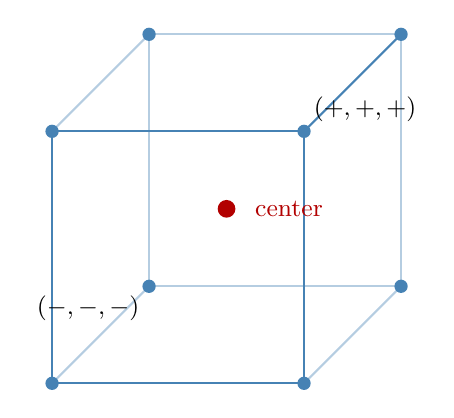
\begin{tikzpicture}[scale=0.8]
  % Factorial cube
  \coordinate (A) at (0,0,0);
  \coordinate (B) at (4,0,0);
  \coordinate (C) at (4,4,0);
  \coordinate (D) at (0,4,0);
  \coordinate (E) at (0,0,4);
  \coordinate (F) at (4,0,4);
  \coordinate (G) at (4,4,4);
  \coordinate (H) at (0,4,4);

  % Back faces
  \draw[thick, steelblue!40] (A) -- (B) -- (C) -- (D) -- cycle;
  \draw[thick, steelblue!40] (A) -- (E);
  \draw[thick, steelblue!40] (B) -- (F);
  \draw[thick, steelblue!40] (D) -- (H);

  % Front faces
  \draw[thick, steelblue] (E) -- (F) -- (G) -- (H) -- cycle;
  \draw[thick, steelblue] (C) -- (G);

  % Corner points
  \foreach \p in {A,B,C,D,E,F,G,H}
    \fill[steelblue] (\p) circle (3pt);

  % Center point
  \fill[red!70!black] (2,2,2) circle (4pt);

  % Labels
  \node[below left] at (A) {\small $(-,-,-)$};
  \node[above right] at (G) {\small $(+,+,+)$};
  \node[right, red!70!black] at (2.3,2,2) {\small center};
\end{tikzpicture}

\vspace{2cm}

\vfill
{\large\sffamily First Edition}\\[0.5cm]
{\normalsize 2025}
\end{titlepage}

% ═══════════════════════════════════════════
% COPYRIGHT
% ═══════════════════════════════════════════
\thispagestyle{empty}
\vspace*{\fill}
\begin{center}
\small
\textit{Design of Experiments: A Practical Guide}\\[1em]
First Edition, 2025\\[2em]
This work is released under the MIT License.\\
You are free to copy, modify, and distribute this work.\\[2em]
Typeset in \TeX\ Gyre Termes.\\
Compiled with Lua\LaTeX.
\end{center}
\vspace*{\fill}
\clearpage

% ═══════════════════════════════════════════
% TABLE OF CONTENTS
% ═══════════════════════════════════════════
\tableofcontents

% ═══════════════════════════════════════════
% PREFACE
% ═══════════════════════════════════════════
\chapter*{Preface}
\addcontentsline{toc}{chapter}{Preface}

This book teaches the theory and practice of Design of Experiments (DOE)---a
systematic method for planning experiments that extracts the maximum information
from the minimum number of runs. It is written for engineers, scientists, and
anyone who runs experiments, benchmarks, or tests and wants to do so more
efficiently.

DOE is not new. Ronald Fisher developed the foundations in the 1920s and 1930s
for agricultural experiments at Rothamsted. George Box, Genichi Taguchi, and
others extended it to manufacturing, quality engineering, and process
optimization. Yet the technique remains underused, especially in software
engineering and technology, where practitioners often default to changing one
variable at a time or running exhaustive grid searches.

This guide takes a practical approach. Each chapter introduces the theory you
need, then shows you how to apply it. Mathematical derivations are included
where they build intuition, but the emphasis is on understanding \emph{when} and
\emph{why} to use each technique, not on proofs.

The examples throughout this book can be run using the open-source DOE Helper
Tool that accompanies it. The tool reads a JSON configuration file, generates an
optimized experimental design, produces an executable runner script, and
analyzes the results with statistical summaries, plots, and reports.

\vspace{1em}
\noindent\textit{Who this book is for:}
\begin{itemize}[nosep]
\item Engineers optimizing systems, processes, or software configurations
\item Scientists planning laboratory or field experiments
\item Data scientists evaluating model hyperparameters
\item Quality engineers improving manufacturing processes
\item Anyone who has ever wondered: ``Which of these 10 knobs actually matters?''
\end{itemize}

\noindent\textit{Prerequisites:} Basic familiarity with mean, variance, and
standard deviation. No prior statistics coursework is assumed.

% ═══════════════════════════════════════════
% PART I: FOUNDATIONS
% ═══════════════════════════════════════════
\part{Foundations}

% ───────────────────────────────────────────
\chapter{Why Design of Experiments?}
% ───────────────────────────────────────────

\section{The Cost of Unplanned Experiments}

Every experiment costs something---time, money, materials, compute cycles. A
poorly planned experiment wastes these resources and may lead to wrong
conclusions. A well-designed experiment extracts the maximum learning from each
run.

\begin{example}[The Cake Analogy]
Imagine you are baking a cake and want to make it taste better. You could try
changing the sugar amount, then the oven temperature, then the baking time---one
thing at a time. After dozens of attempts, you might find a decent recipe. But
you would never discover that a \emph{specific combination} of less sugar
\emph{with} higher temperature produces the best result, because you never tested
them together. DOE solves exactly this problem.
\end{example}

Consider a team tuning a database. They have five configuration knobs they
suspect affect performance: buffer pool size, I/O capacity, connection limit,
query cache, and thread pool size. The one-variable-at-a-time (OVAT) approach
would be:

\begin{enumerate}[nosep]
\item Fix all knobs at their defaults.
\item Change buffer pool size. Measure.
\item Reset buffer pool. Change I/O capacity. Measure.
\item Continue for each knob.
\end{enumerate}

This requires at least 10 runs (2 per knob) and only measures each knob's
effect \emph{in isolation, at the default settings of every other knob}. It
tells you nothing about how the knobs interact.

A Plackett--Burman screening design tests all five knobs in just 8 runs and
estimates every main effect simultaneously. A full factorial on the two most
important knobs then takes 4 more runs and reveals their interaction. Twelve
runs total, and you know more than OVAT would teach you in fifty.

\section{The Three Principles of DOE}

Fisher established three principles that remain the foundation of every
well-designed experiment:

\subsection{Randomization}

\begin{keypoint}[Randomization]
Randomly assign the order in which experimental runs are performed to protect
against unknown lurking variables.
\end{keypoint}

If you run all low-temperature experiments in the morning and all
high-temperature experiments in the afternoon, any morning-to-afternoon drift
(ambient temperature, operator alertness, equipment warm-up) becomes confounded
with your temperature factor. You cannot tell whether the observed difference is
due to temperature or time of day.

Randomization does not eliminate lurking variables---it distributes their effects
equally across all treatments, on average. This ensures that the statistical
tests remain valid.

Mathematically, if $Y_{ij}$ is the response for factor level $i$ in run order
$j$, and there is a time trend $\delta_j$, then without randomization:
\[
E[Y_{ij}] = \mu + \tau_i + \delta_j
\]
where $\tau_i$ and $\delta_j$ may be confounded. With randomization, $\delta_j$
is equally likely to affect any treatment, so:
\[
E[\bar{Y}_{i\cdot}] = \mu + \tau_i
\]
and the time trend averages out.

\subsection{Replication}

\begin{keypoint}[Replication]
Repeat experimental runs to estimate experimental error and increase the
precision of effect estimates.
\end{keypoint}

A single run at each factor combination tells you the response at that
combination, but it does not tell you how much that response varies. Without an
estimate of variability, you cannot determine whether an observed difference is
real or just noise.

Replication provides:
\begin{itemize}[nosep]
\item An estimate of the experimental error variance $\sigma^2$
\item More precise estimates of effects (standard error decreases as $1/\sqrt{n}$)
\item The ability to construct confidence intervals and perform significance tests
\end{itemize}

\begin{warning}[Replication vs.\ Repetition]
\textbf{Replication} means independently setting up and running the experiment
again. \textbf{Repetition} means measuring the same setup multiple times.
Repetition estimates measurement error, but replication estimates the full
experimental error, including setup variation. DOE requires replication.
\end{warning}

\subsection{Blocking}

\begin{keypoint}[Blocking]
Group experimental runs into blocks of similar conditions to remove known sources
of variation from the experimental error.
\end{keypoint}

If you must run experiments over two days, make each day a block. Within each
block (day), randomize the run order. The day-to-day variation is then
accounted for in the analysis and does not inflate the error estimate.

The model becomes:
\[
Y_{ijk} = \mu + \tau_i + \beta_j + \epsilon_{ijk}
\]
where $\beta_j$ is the block effect. Because blocks are orthogonal to
treatments in a balanced design, the treatment effects $\tau_i$ are estimated
without bias.

\section{The OVAT Trap: A Quantitative Example}

Suppose the true relationship between yield and two factors (temperature $T$ and
pressure $P$) is:
\[
Y = 50 + 10T + 5P + 8TP + \epsilon
\]
where $T, P \in \{-1, +1\}$ (coded levels) and $\epsilon \sim N(0, 1)$.

\subsection{OVAT Analysis}

\begin{enumerate}[nosep]
\item Run at $T=-1, P=-1$: $Y = 50 - 10 - 5 + 8 = 43$
\item Change $T$ to $+1$: $Y = 50 + 10 - 5 - 8 = 47$
\item Conclude: Temperature effect $= 47 - 43 = 4$
\end{enumerate}

But the true main effect of temperature is $+10$, not $+4$! The OVAT estimate is
biased because it was measured at $P=-1$, where the interaction $TP$ reduces
temperature's apparent effect. At $P=+1$, the temperature effect would appear as $+18$.

\subsection{Factorial Analysis}

A $2^2$ factorial runs all four combinations:

\begin{center}
\begin{tabular}{cccc}
\toprule
Run & $T$ & $P$ & $Y$ (expected) \\
\midrule
1 & $-1$ & $-1$ & 43 \\
2 & $+1$ & $-1$ & 47 \\
3 & $-1$ & $+1$ & 37 \\
4 & $+1$ & $+1$ & 73 \\
\bottomrule
\end{tabular}
\end{center}

\noindent Main effect of $T$:
\[
\text{ME}_T = \frac{(Y_2 + Y_4)}{2} - \frac{(Y_1 + Y_3)}{2}
= \frac{47 + 73}{2} - \frac{43 + 37}{2} = 60 - 40 = 20
\]

Wait---the formula gives 20, but we said the coefficient was 10. In the effects
model, the main effect is \emph{twice} the coefficient because we move from
$-1$ to $+1$ (a change of 2 units). So $\text{ME}_T / 2 = 10$, exactly the
true coefficient.

The interaction effect:
\[
\text{IE}_{TP} = \frac{(Y_1 + Y_4)}{2} - \frac{(Y_2 + Y_3)}{2}
= \frac{43 + 73}{2} - \frac{47 + 37}{2} = 58 - 42 = 16
\]

Again, $\text{IE}_{TP} / 2 = 8$, the true interaction coefficient. The factorial
design correctly estimates both effects and their interaction, using the same
number of runs where each piece of data contributes to every estimate.

\begin{keypoint}[Hidden Replication in Factorials]
In a $2^k$ factorial, every effect estimate uses \emph{all} $2^k$ observations.
Each observation plays a role in estimating every effect. This is why factorials
are so efficient---there is no wasted data.
\end{keypoint}

\section{A Concrete Example: Web Server Tuning}

This example makes the OVAT trap viscerally clear. Suppose you are optimizing
a web server and suspect two things matter: \textbf{thread count} (10 or 100)
and \textbf{cache size} (64\,MB or 512\,MB). The true relationship (which you
do not know yet) is:

\begin{center}
\begin{tabular}{ccr}
\toprule
Thread Count & Cache Size & Throughput (req/sec) \\
\midrule
10 & 64\,MB & 500 \\
100 & 64\,MB & 600 \\
10 & 512\,MB & 700 \\
100 & 512\,MB & 1400 \\
\bottomrule
\end{tabular}
\end{center}

\subsection{OVAT Gets the Wrong Answer}

Starting at (10 threads, 64\,MB cache):
\begin{enumerate}[nosep]
\item Change threads to 100, keep cache at 64\,MB $\to$ throughput goes from
      500 to 600. \emph{Conclusion: threads help a little (+100).}
\item Reset threads to 10. Change cache to 512\,MB $\to$ throughput goes from
      500 to 700. \emph{Conclusion: cache helps more (+200).}
\item Final recommendation: use 512\,MB cache. Predicted throughput: 700.
\end{enumerate}

\subsection{DOE Gets the Right Answer}

A $2^2$ full factorial tests all four combinations:
\begin{itemize}[nosep]
\item Main effect of threads: $\frac{600 + 1400}{2} - \frac{500 + 700}{2}
      = 1000 - 600 = \mathbf{+400}$
\item Main effect of cache: $\frac{700 + 1400}{2} - \frac{500 + 600}{2}
      = 1050 - 550 = \mathbf{+500}$
\item Interaction effect: $\mathbf{+500}$ (threads and cache amplify each other)
\item Recommendation: use \emph{both} 100 threads and 512\,MB cache.
      Throughput: \textbf{1400}.
\end{itemize}

Same number of experiments. Completely different---and correct---conclusion.
The OVAT approach missed the interaction entirely and left 700 req/sec of
throughput on the table.

\begin{warning}[Interactions Are the Rule, Not the Exception]
In the web server example, the cache is only truly effective when there are
enough threads to use it. This kind of synergy is extremely common in real
systems---database buffer pools that only help with high I/O capacity, compiler
optimizations that only matter with specific architecture targets, or machine
learning learning rates that only work with certain batch sizes.
\end{warning}

\section{DOE in Everyday Life}

The logic of DOE is not confined to laboratories or data centers. You use it---or
fail to use it---whenever you try to improve anything with multiple knobs to turn.

\begin{example}[Cooking: Testing Seasoning Combinations]
Suppose you are perfecting a pasta sauce and want to know how much \textbf{salt},
\textbf{garlic}, and \textbf{chili flake} to add. You could test each seasoning
one at a time, holding the others constant. But what if garlic only shines when
paired with enough salt to bring out its flavor? A factorial approach---testing
all combinations of low/high for each seasoning---lets you discover that the
magic is in the \emph{combination} of moderate salt with generous garlic, while
chili flake barely matters. Eight small batches tell you more than twenty
one-at-a-time tastings.
\end{example}

\begin{example}[Gardening: Fertilizer, Watering, and Sunlight]
A gardener wants bigger tomatoes. The controllable factors are
\textbf{fertilizer} (low vs.\ high), \textbf{watering frequency}
(daily vs.\ every other day), and \textbf{sunlight exposure} (partial shade
vs.\ full sun). Instead of changing one factor per growing season (which would
take three seasons), the gardener plants eight small plots---one for each
combination---in the same season. The result: fertilizer has a huge effect, but
\emph{only} when combined with daily watering. Full sun helps regardless. Two
weeks of harvest data replace three years of guesswork.
\end{example}

\begin{example}[Shopping: Comparing Products Across Multiple Criteria]
When buying a laptop, you care about \textbf{price}, \textbf{battery life}, and
\textbf{weight}. Sorting a comparison table by just one criterion (say, price)
hides the trade-offs. A DOE mindset asks: ``Which criterion has the biggest
effect on my satisfaction?'' and ``Do any criteria interact?'' (e.g., you
only care about weight if battery life is long enough to leave the charger at
home). Thinking in terms of factors, levels, and interactions helps you make
multi-criteria decisions systematically, even outside a formal experiment.
\end{example}


% ───────────────────────────────────────────
\chapter{Statistical Foundations}
% ───────────────────────────────────────────

\section{The Linear Model}

Before we write down any math, let us understand what we are doing in plain
English. We are trying to build a simple equation that predicts our response
from the factor settings. Think of it as:

\medskip
\centerline{Result = (baseline) + (contribution from factor A) + (contribution from factor B)}
\centerline{+ (how A and B work together) + (random noise)}
\medskip

\noindent
Each factor either pushes the result up or pulls it down by some amount, and
the interaction term captures any synergy or conflict between factors. The math
below just makes this precise.

At the heart of DOE analysis is the general linear model. For a single response
$Y$ with $k$ factors:
\[
Y = \beta_0 + \sum_{i=1}^{k} \beta_i x_i
+ \sum_{i<j} \beta_{ij} x_i x_j + \epsilon
\]
where:
\begin{itemize}[nosep]
\item $\beta_0$ is the grand mean (intercept)
\item $\beta_i$ are the main effect coefficients
\item $\beta_{ij}$ are the interaction coefficients
\item $x_i \in \{-1, +1\}$ are the coded factor levels
\item $\epsilon \sim N(0, \sigma^2)$ is the random error
\end{itemize}

For a quadratic (response surface) model, add squared terms:
\[
Y = \beta_0 + \sum_{i=1}^{k} \beta_i x_i
+ \sum_{i<j} \beta_{ij} x_i x_j
+ \sum_{i=1}^{k} \beta_{ii} x_i^2 + \epsilon
\]

\section{Coded Variables}

Coding is just putting all factors on the same scale. If one factor is measured
in degrees (150--200) and another in bars (2--6), their raw numbers are not
comparable. A coefficient of 5 for temperature and 5 for pressure in raw units
would \emph{not} mean they have the same importance, because a 50-degree change
is very different from a 4-bar change. Coding transforms both factors to a $-1$
to $+1$ scale, so a coefficient of 5 for temperature and 5 for pressure
genuinely means they have the same effect on the response.

Factor levels are coded to simplify calculations and make effects directly
comparable. For a continuous factor with low value $L$ and high value $H$:
\[
x = \frac{\text{actual value} - \frac{L+H}{2}}{\frac{H-L}{2}}
\]

This maps $L \to -1$ and $H \to +1$. The center is at $x=0$. All factors are on
the same scale, so their coefficients are directly comparable---a coefficient of
10 means the same magnitude of effect regardless of whether the factor is
measured in degrees or bars.

\section{Estimating Effects}

\subsection{Main Effects}

The main effect of factor $A$ is the difference in the average response when $A$
is at its high level versus its low level:
\[
\text{ME}_A = \bar{Y}_{A+} - \bar{Y}_{A-}
\]

In a $2^k$ design, each average uses half the total runs, so the standard error
of a main effect is:
\[
\text{SE}(\text{ME}_A) = \sqrt{\frac{4s^2}{N}}
= \frac{2s}{\sqrt{N}}
\]
where $s^2$ is the pooled variance estimate and $N$ is the total number of runs.

\begin{example}[Calculating a Main Effect by Hand]
Suppose we have a $2^2$ design with factors $A$ and $B$, and the response values are:
$Y(A{-}, B{-}) = 20$, $Y(A{+}, B{-}) = 40$, $Y(A{-}, B{+}) = 30$, $Y(A{+}, B{+}) = 60$.

Main effect of $A$ = average when $A$ is high $-$ average when $A$ is low:
\[
\text{ME}_A = \frac{40 + 60}{2} - \frac{20 + 30}{2} = 50 - 25 = +25
\]

This means changing $A$ from low to high increases the response by 25 units, on average.
\end{example}

\subsection{Interaction Effects}

The two-factor interaction $AB$ measures whether the effect of $A$ depends on the
level of $B$. Compute it as:
\[
\text{IE}_{AB} = \frac{1}{2}\bigl[(\text{effect of } A \text{ at } B_{+})
- (\text{effect of } A \text{ at } B_{-})\bigr]
\]

Equivalently, in a $2^k$ design:
\[
\text{IE}_{AB} = \bar{Y}_{\text{concordant}} - \bar{Y}_{\text{discordant}}
\]
where ``concordant'' runs have $A$ and $B$ both high or both low, and
``discordant'' runs have one high and one low.

\begin{example}[Calculating an Interaction by Hand]
Using the same $2^2$ data as before ($Y(A{-}, B{-}) = 20$, $Y(A{+}, B{-}) = 40$,
$Y(A{-}, B{+}) = 30$, $Y(A{+}, B{+}) = 60$):

Effect of $A$ when $B$ is low $= 40 - 20 = 20$.

Effect of $A$ when $B$ is high $= 60 - 30 = 30$.

The interaction $AB = (30 - 20)/2 = +5$.

This positive interaction means $A$ is MORE effective when $B$ is high.
The factors amplify each other.

If the interaction were negative, $A$ would be LESS effective at $B$-high
(the factors would cancel each other).
\end{example}

\subsection{Percentage Contribution}

To rank factors by importance, compute each factor's percentage contribution:
\[
\text{PC}_i = \frac{|\text{ME}_i|}{\sum_{j=1}^{k} |\text{ME}_j|} \times 100\%
\]

This appears on the Pareto chart. The ``vital few'' factors typically account
for 70--80\% of the total effect magnitude.

\section{Confidence Intervals}

A 95\% confidence interval for a main effect is:
\[
\text{ME}_A \pm t_{\alpha/2, \nu} \cdot \text{SE}(\text{ME}_A)
\]
where $t_{\alpha/2, \nu}$ is the critical value from the $t$-distribution with
$\nu$ degrees of freedom. If the interval contains zero, the effect is not
statistically significant at the 5\% level.

For a two-level design with $n_-$ and $n_+$ observations at the low and high
levels respectively:
\[
\text{SE}(\text{ME}_A) = s_p \sqrt{\frac{1}{n_-} + \frac{1}{n_+}}
\]
where $s_p$ is the pooled standard deviation:
\[
s_p = \sqrt{\frac{(n_- - 1)s_-^2 + (n_+ - 1)s_+^2}{n_- + n_+ - 2}}
\]

\section{Analysis of Variance (ANOVA)}

ANOVA answers a simple question: ``How much of the total variation in my results
is caused by each factor, and how much is just noise?'' It splits the total
variation into pieces---like splitting a pie chart---so you can see which factors
account for the biggest slices. If temperature accounts for 60\% of the
variation, pressure for 15\%, and the remaining 25\% is unexplained noise, you
know exactly where to focus your optimization effort.

ANOVA decomposes the total variation in the response into components attributable
to each factor, their interactions, and the residual error:
\[
\text{SS}_{\text{Total}} = \sum_i \text{SS}_{A_i}
+ \sum_{i<j} \text{SS}_{A_iA_j} + \text{SS}_{\text{Error}}
\]

For a main effect in a $2^k$ design:
\[
\text{SS}_A = \frac{N}{4} \cdot \text{ME}_A^2
\]

The $F$-statistic for testing whether factor $A$ has a significant effect is:
\[
F_A = \frac{\text{SS}_A / 1}{\text{SS}_{\text{Error}} / \nu_E}
= \frac{\text{MS}_A}{\text{MS}_E}
\]

If $F_A > F_{\alpha, 1, \nu_E}$, reject the null hypothesis that factor $A$ has
no effect.

\section{The $R^2$ Statistic}

$R^2$ measures the proportion of variance in the response explained by the
model:
\[
R^2 = 1 - \frac{\text{SS}_{\text{Error}}}{\text{SS}_{\text{Total}}}
\]

The adjusted $R^2$ penalizes for model complexity:
\[
R^2_{\text{adj}} = 1 - \frac{\text{SS}_{\text{Error}} / \nu_E}
{\text{SS}_{\text{Total}} / \nu_T}
\]

An $R^2$ near 1.0 means the model explains nearly all the variation. An $R^2$
below 0.7 suggests important factors or relationships are missing from the
model.

\begin{warning}[When High $R^2$ Is Misleading]
$R^2$ can be artificially inflated by having many model terms relative to data
points. If you fit a quadratic model with 10 parameters to 12 data points,
$R^2$ will be high even if the model is meaningless.

Always compare $R^2$ and $R^2_{\text{adj}}$. A large gap (e.g., $R^2 = 0.95$
but $R^2_{\text{adj}} = 0.75$) signals overfitting.

Rule of thumb: you need at least $1.5\times$ as many data points as model
parameters.
\end{warning}


% ═══════════════════════════════════════════
% PART II: DESIGN TYPES
% ═══════════════════════════════════════════
\part{Design Types}

% ───────────────────────────────────────────
\chapter{Full Factorial Designs}
% ───────────────────────────────────────────

\section{The $2^k$ Factorial}

The $2^k$ full factorial design tests every combination of $k$ factors at 2
levels each. It is the most complete two-level design: it estimates all main
effects, all two-factor interactions, and all higher-order interactions with no
confounding.

\subsection{Run Count}

\begin{center}
\begin{tabular}{ccl}
\toprule
Factors ($k$) & Runs ($2^k$) & Notes \\
\midrule
2 & 4  & Minimum useful design \\
3 & 8  & Very practical \\
4 & 16 & Still manageable \\
5 & 32 & Getting expensive \\
6 & 64 & Consider fractional \\
7 & 128 & Fractional almost always better \\
\bottomrule
\end{tabular}
\end{center}

\subsection{The Design Matrix}

For a $2^3$ design with factors $A$, $B$, $C$:

\begin{center}
\begin{tabular}{cccccccc}
\toprule
Run & $A$ & $B$ & $C$ & $AB$ & $AC$ & $BC$ & $ABC$ \\
\midrule
1 & $-$ & $-$ & $-$ & $+$ & $+$ & $+$ & $-$ \\
2 & $+$ & $-$ & $-$ & $-$ & $-$ & $+$ & $+$ \\
3 & $-$ & $+$ & $-$ & $-$ & $+$ & $-$ & $+$ \\
4 & $+$ & $+$ & $-$ & $+$ & $-$ & $-$ & $-$ \\
5 & $-$ & $-$ & $+$ & $+$ & $-$ & $-$ & $+$ \\
6 & $+$ & $-$ & $+$ & $-$ & $+$ & $-$ & $-$ \\
7 & $-$ & $+$ & $+$ & $-$ & $-$ & $+$ & $-$ \\
8 & $+$ & $+$ & $+$ & $+$ & $+$ & $+$ & $+$ \\
\bottomrule
\end{tabular}
\end{center}

The interaction columns are computed by multiplying the corresponding main
effect columns element-wise. This orthogonality property---every column has an
equal number of $+$ and $-$ signs, and the inner product of any two columns is
zero---is what makes the effect estimates independent and unbiased.

\subsection{Geometric Interpretation}

\begin{center}
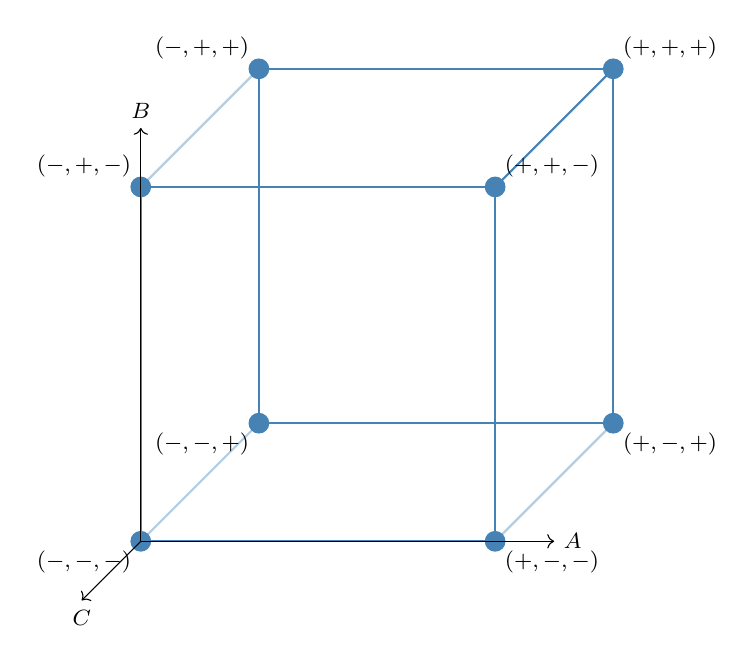
\begin{tikzpicture}[scale=1.5]
  % Cube
  \coordinate (A) at (0,0);
  \coordinate (B) at (3,0);
  \coordinate (C) at (3,3);
  \coordinate (D) at (0,3);
  \coordinate (E) at (1,1);
  \coordinate (F) at (4,1);
  \coordinate (G) at (4,4);
  \coordinate (H) at (1,4);

  \draw[thick, steelblue!40] (A) -- (E) (B) -- (F) (D) -- (H);
  \draw[thick, steelblue] (A) -- (B) -- (C) -- (D) -- cycle;
  \draw[thick, steelblue] (E) -- (F) -- (G) -- (H) -- cycle;
  \draw[thick, steelblue] (C) -- (G);

  \foreach \p in {A,B,C,D,E,F,G,H}
    \fill[steelblue] (\p) circle (2.5pt);

  \node[below left] at (A) {\footnotesize $(-,-,-)$};
  \node[below right] at (B) {\footnotesize $(+,-,-)$};
  \node[above right] at (C) {\footnotesize $(+,+,-)$};
  \node[above left] at (D) {\footnotesize $(-,+,-)$};
  \node[below left] at (E) {\footnotesize $(-,-,+)$};
  \node[below right] at (F) {\footnotesize $(+,-,+)$};
  \node[above right] at (G) {\footnotesize $(+,+,+)$};
  \node[above left] at (H) {\footnotesize $(-,+,+)$};

  \draw[->] (A) -- +(-0.5, -0.5) node[below] {\footnotesize $C$};
  \draw[->] (A) -- +(3.5, 0) node[right] {\footnotesize $A$};
  \draw[->] (A) -- +(0, 3.5) node[above] {\footnotesize $B$};
\end{tikzpicture}
\captionof{figure}{A $2^3$ full factorial as a cube. Each vertex is an
experimental run. The main effect of $A$ is the average of the four right-face
responses minus the average of the four left-face responses.}
\end{center}

\section{Mixed-Level Factorials}

Full factorials are not limited to two levels. A $3 \times 2 \times 4$ design
tests one factor at 3 levels, one at 2, and one at 4, yielding $3 \times 2
\times 4 = 24$ runs. The analysis uses the range of level means (maximum mean
minus minimum mean) instead of the simple high-minus-low formula.

\section{When to Use Full Factorials}

\begin{itemize}[nosep]
\item 2--4 factors: almost always the right choice
\item You need to estimate all interactions, not just main effects
\item Runs are cheap relative to the information gained
\item You suspect important interactions exist
\end{itemize}


\section{Worked Example: A Complete $2^3$ Analysis}

Consider a packaging engineer testing three factors that affect the seal
strength (in Newtons) of a heat-sealed pouch:

\begin{itemize}[nosep]
\item \textbf{A}: Seal temperature ($-1$ = 150\textdegree C, $+1$ = 190\textdegree C)
\item \textbf{B}: Pressure ($-1$ = 2\,bar, $+1$ = 5\,bar)
\item \textbf{C}: Dwell time ($-1$ = 0.5\,s, $+1$ = 1.5\,s)
\end{itemize}

\noindent A $2^3$ full factorial requires $8$ runs. The engineer randomizes the
run order, performs the experiment, and records the following seal strength
values:

\begin{center}
\begin{tabular}{ccccr}
\toprule
Run & $A$ (temp) & $B$ (pressure) & $C$ (dwell) & Seal Strength (N) \\
\midrule
1 & $-1$ & $-1$ & $-1$ & 28.4 \\
2 & $+1$ & $-1$ & $-1$ & 39.1 \\
3 & $-1$ & $+1$ & $-1$ & 31.6 \\
4 & $+1$ & $+1$ & $-1$ & 46.5 \\
5 & $-1$ & $-1$ & $+1$ & 29.8 \\
6 & $+1$ & $-1$ & $+1$ & 40.7 \\
7 & $-1$ & $+1$ & $+1$ & 33.0 \\
8 & $+1$ & $+1$ & $+1$ & 48.3 \\
\bottomrule
\end{tabular}
\end{center}

The grand mean is:
\[
\bar{y} = \frac{28.4 + 39.1 + 31.6 + 46.5 + 29.8 + 40.7 + 33.0 + 48.3}{8}
= \frac{297.4}{8} = 37.175 \text{ N}
\]

\subsection{Main Effect of A (Seal Temperature)}

Average at $A = +1$: $\bar{y}_{A+} = (39.1 + 46.5 + 40.7 + 48.3)/4 = 43.65$

Average at $A = -1$: $\bar{y}_{A-} = (28.4 + 31.6 + 29.8 + 33.0)/4 = 30.70$

\[
\text{ME}_A = 43.65 - 30.70 = +12.95 \text{ N}
\]

Increasing temperature from 150\textdegree C to 190\textdegree C raises seal
strength by an average of 12.95\,N.

\subsection{Main Effect of B (Pressure)}

Average at $B = +1$: $\bar{y}_{B+} = (31.6 + 46.5 + 33.0 + 48.3)/4 = 39.85$

Average at $B = -1$: $\bar{y}_{B-} = (28.4 + 39.1 + 29.8 + 40.7)/4 = 34.50$

\[
\text{ME}_B = 39.85 - 34.50 = +5.35 \text{ N}
\]

\subsection{Main Effect of C (Dwell Time)}

Average at $C = +1$: $\bar{y}_{C+} = (29.8 + 40.7 + 33.0 + 48.3)/4 = 37.95$

Average at $C = -1$: $\bar{y}_{C-} = (28.4 + 39.1 + 31.6 + 46.5)/4 = 36.40$

\[
\text{ME}_C = 37.95 - 36.40 = +1.55 \text{ N}
\]

\subsection{The AB Interaction (Temperature $\times$ Pressure)}

To calculate the $AB$ interaction, we compare runs where $A$ and $B$ have the
same sign (concordant) against runs where they have opposite signs (discordant):

Concordant ($AB = +1$): runs 1, 4, 5, 8 $\to$ $\bar{y} = (28.4 + 46.5 + 29.8 + 48.3)/4 = 38.25$

Discordant ($AB = -1$): runs 2, 3, 6, 7 $\to$ $\bar{y} = (39.1 + 31.6 + 40.7 + 33.0)/4 = 36.10$

\[
\text{IE}_{AB} = 38.25 - 36.10 = +2.15 \text{ N}
\]

This positive interaction means that the combined effect of high temperature
\emph{and} high pressure is greater than the sum of their individual effects.
Temperature works even better at high pressure.

\subsection{Summary of All Effects}

\begin{center}
\begin{tabular}{lrr}
\toprule
Effect & Magnitude (N) & Cumulative \% \\
\midrule
A (temperature) & 12.95 & 58.8\% \\
B (pressure) & 5.35 & 83.1\% \\
AB (temp $\times$ pressure) & 2.15 & 92.8\% \\
C (dwell time) & 1.55 & 99.9\% \\
\bottomrule
\end{tabular}
\end{center}

Seal temperature has by far the largest effect ($+12.95$\,N). The $AB$
interaction is moderate ($+2.15$\,N), meaning temperature works better at high
pressure---the polymer chains flow more readily into good contact when both heat
and pressure are elevated. Dwell time has a negligible effect ($+1.55$\,N) and
can be set to the short value (0.5\,s) to minimize cycle time and maximize
production throughput.

\section{Adding Center Points}

A $2^k$ full factorial tests only the corners of the factor space. If the true
relationship between a factor and the response is curved (quadratic), the
factorial design cannot detect it. \emph{Center points} address this limitation
at minimal cost.

\subsection{What Are Center Points?}

Center points are experimental runs performed at the midpoint of every factor
simultaneously. For the packaging example above, a center point would be:
$\text{temp} = 170$\textdegree C, $\text{pressure} = 3.5$\,bar,
$\text{dwell} = 1.0$\,s.

Typically 3--5 center point replicates are added to the factorial design. These
runs serve two purposes: they provide an independent estimate of pure error
(since they are replicates at the same settings), and they allow a test for
curvature.

\subsection{Testing for Curvature}

The curvature effect is defined as the difference between the average of the
center points and the average of the factorial (corner) points:
\[
\text{Curvature} = \bar{y}_{\text{center}} - \bar{y}_{\text{factorial}}
\]

If this difference is close to zero, the response surface is approximately
planar over the tested region, and the factorial model is adequate. If the
difference is large and statistically significant, curvature exists---the
optimum is not at a corner of the design space but somewhere in the interior.

To test significance, compute:
\[
t = \frac{\bar{y}_{\text{center}} - \bar{y}_{\text{factorial}}}
{s_p \sqrt{\dfrac{1}{n_c} + \dfrac{1}{n_f}}}
\]
where $n_c$ is the number of center points, $n_f$ is the number of factorial
points, and $s_p$ is the pooled standard deviation estimated from the center
point replicates.

\subsection{When Curvature Is Detected}

If the curvature test is significant, the $2^k$ factorial model is not adequate
to describe the response surface. The next step is to augment the design into a
response surface design:

\begin{itemize}[nosep]
\item Add axial (star) points to create a \textbf{Central Composite Design}
      (CCD). The existing factorial points and center points are reused; only the
      $2k$ star points need to be run.
\item Alternatively, run a \textbf{Box--Behnken} design from scratch if the
      axial points fall outside feasible operating conditions.
\end{itemize}

This sequential approach is efficient: you invest the minimum runs (factorial +
center points) first, and only escalate to a full response surface design when
the data demand it.

% ───────────────────────────────────────────
\chapter{Fractional Factorial Designs}
% ───────────────────────────────────────────

\section{The Problem of Exponential Growth}

As the number of factors increases, full factorials become impractical. With 7
factors at 2 levels, a full factorial requires $2^7 = 128$ runs. But in
practice, the \emph{effect sparsity principle} states that most of the variation
is explained by main effects and low-order interactions. Higher-order
interactions ($ABC$, $ABCD$, etc.) are usually negligible.

Fractional factorials exploit this by deliberately confounding higher-order
interactions with main effects or lower-order interactions, trading information
about unlikely-to-matter effects for a dramatic reduction in runs.

\section{The $2^{k-p}$ Design}

A $2^{k-p}$ fractional factorial uses $2^{k-p}$ runs to study $k$ factors. The
integer $p$ is the \emph{degree of fractionation}: each increase in $p$ halves
the number of runs.

\begin{center}
\begin{tabular}{cccc}
\toprule
Design & Factors & Runs & Fraction \\
\midrule
$2^{4-1}$ & 4 & 8 & $\frac{1}{2}$ \\
$2^{5-1}$ & 5 & 16 & $\frac{1}{2}$ \\
$2^{5-2}$ & 5 & 8 & $\frac{1}{4}$ \\
$2^{7-4}$ & 7 & 8 & $\frac{1}{16}$ \\
\bottomrule
\end{tabular}
\end{center}

\section{Resolution}

The \emph{resolution} of a fractional factorial describes the severity of the
confounding:

\begin{center}
\begin{tabular}{cl}
\toprule
Resolution & Confounding Pattern \\
\midrule
III & Main effects aliased with 2-factor interactions \\
IV & Main effects clear; 2FIs aliased with other 2FIs \\
V & Main effects and 2FIs clear; 2FIs aliased with 3FIs \\
\bottomrule
\end{tabular}
\end{center}

\begin{keypoint}[Choosing Resolution]
Use Resolution III for initial screening (many factors, few runs). Use
Resolution IV or V when you suspect important 2-factor interactions and want
to estimate them separately from main effects. The higher the resolution, the
more runs are required.
\end{keypoint}

\section{Generator Strings and Aliasing}

A fractional factorial is defined by its \emph{generators}---the rules that
assign aliased factor columns. For a $2^{5-2}_{III}$ design, the base factors
are $A$, $B$, $C$ (requiring $2^3 = 8$ runs), and the two additional factors
are defined as:
\begin{align*}
D &= AB \\
E &= AC
\end{align*}

The \emph{defining relation} is the set of column products equal to $I$ (the
identity):
\[
I = ABD = ACE = BCDE
\]

Any two columns whose product appears in the defining relation are aliased
(confounded). For example, $A = BD = CE$ and $B = AD = CDE$.

\section{Practical Guidance}

\begin{enumerate}[nosep]
\item If you have $k \leq 4$ factors, use a full factorial.
\item If $5 \leq k \leq 7$, use a Resolution IV or V fraction.
\item If $k > 7$ and you are screening, use Resolution III or a Plackett--Burman.
\item Always check the alias structure before running the experiment to ensure
      the effects you care about are not aliased with each other.
\end{enumerate}


\section{Worked Example: A $2^{4-1}$ Half Fraction}

Suppose we want to study 4 factors in only 8 runs instead of the 16 required by
a full $2^4$ factorial. We construct a $2^{4-1}$ design by starting with a full
$2^3$ factorial in factors $A$, $B$, and $C$ (the base design), then defining
the fourth factor as:
\[
D = ABC
\]

This is the \emph{generator} of the design. It means that in each run, the
level of $D$ is set equal to the product of the levels of $A$, $B$, and $C$.
The defining relation is $I = ABCD$, which tells us that the column of all
$+1$s (the identity $I$) is identical to the element-wise product $ABCD$.

The complete design matrix is:

\begin{center}
\begin{tabular}{ccccc}
\toprule
Run & $A$ & $B$ & $C$ & $D = ABC$ \\
\midrule
1 & $-$ & $-$ & $-$ & $-$ \\
2 & $+$ & $-$ & $-$ & $+$ \\
3 & $-$ & $+$ & $-$ & $+$ \\
4 & $+$ & $+$ & $-$ & $-$ \\
5 & $-$ & $-$ & $+$ & $+$ \\
6 & $+$ & $-$ & $+$ & $-$ \\
7 & $-$ & $+$ & $+$ & $-$ \\
8 & $+$ & $+$ & $+$ & $+$ \\
\bottomrule
\end{tabular}
\end{center}

\subsection{The Alias Structure}

From the defining relation $I = ABCD$, we can find every alias pair by
multiplying each effect by $ABCD$:

\begin{center}
\begin{tabular}{lcl}
\toprule
Effect & is aliased with & Alias \\
\midrule
$A$ & $\leftrightarrow$ & $BCD$ \\
$B$ & $\leftrightarrow$ & $ACD$ \\
$C$ & $\leftrightarrow$ & $ABD$ \\
$D$ & $\leftrightarrow$ & $ABC$ \\
$AB$ & $\leftrightarrow$ & $CD$ \\
$AC$ & $\leftrightarrow$ & $BD$ \\
$BC$ & $\leftrightarrow$ & $AD$ \\
\bottomrule
\end{tabular}
\end{center}

This is a \textbf{Resolution~IV} design. Main effects ($A$, $B$, $C$, $D$) are
aliased with three-factor interactions ($BCD$, $ACD$, $ABD$, $ABC$). By the
effect sparsity principle, three-factor interactions are almost always
negligible, so the main effect estimates are trustworthy. However, two-factor
interactions are aliased with other two-factor interactions ($AB = CD$,
$AC = BD$, $BC = AD$), so if we observe a large ``$AB$'' effect, we cannot tell
whether it is due to the $AB$ interaction, the $CD$ interaction, or some
combination of both.

\subsection{Response Data and Main Effects}

Suppose the four factors are settings of a web application:
\begin{itemize}[nosep]
\item $A$: Database connection pool size (10 vs.\ 50)
\item $B$: API timeout (1\,s vs.\ 5\,s)
\item $C$: Cache enabled (no vs.\ yes)
\item $D$: Compression enabled (no vs.\ yes)
\end{itemize}

\noindent Running the 8 experiments yields the following response times (ms):

\begin{center}
\begin{tabular}{ccccccr}
\toprule
Run & $A$ & $B$ & $C$ & $D$ & & Response (ms) \\
\midrule
1 & $-$ & $-$ & $-$ & $-$ & & 245 \\
2 & $+$ & $-$ & $-$ & $+$ & & 198 \\
3 & $-$ & $+$ & $-$ & $+$ & & 231 \\
4 & $+$ & $+$ & $-$ & $-$ & & 187 \\
5 & $-$ & $-$ & $+$ & $+$ & & 178 \\
6 & $+$ & $-$ & $+$ & $-$ & & 142 \\
7 & $-$ & $+$ & $+$ & $-$ & & 165 \\
8 & $+$ & $+$ & $+$ & $+$ & & 121 \\
\bottomrule
\end{tabular}
\end{center}

Computing main effects:
\begin{align*}
\text{ME}_A &= \frac{198+187+142+121}{4} - \frac{245+231+178+165}{4}
= 162.0 - 204.75 = -42.75 \text{ ms} \\
\text{ME}_B &= \frac{231+187+165+121}{4} - \frac{245+198+178+142}{4}
= 176.0 - 190.75 = -14.75 \text{ ms} \\
\text{ME}_C &= \frac{178+142+165+121}{4} - \frac{245+198+231+187}{4}
= 151.5 - 215.25 = -63.75 \text{ ms} \\
\text{ME}_D &= \frac{198+231+178+121}{4} - \frac{245+187+142+165}{4}
= 182.0 - 184.75 = -2.75 \text{ ms}
\end{align*}

Cache ($C$) has the largest effect: enabling it reduces response time by
63.75\,ms on average. Connection pool size ($A$) is the second most important
factor at $-42.75$\,ms. We can trust these main effect estimates because their
aliases---the three-factor interactions $ABD$ and $BCD$---are almost certainly
negligible. Compression ($D$) has essentially no effect ($-2.75$\,ms) and can
be set to whichever value minimizes CPU usage.

\section{Foldover: Recovering Lost Information}

Sometimes a Resolution~III design is the only option within the run budget.
In such a design, main effects are aliased with two-factor interactions
(e.g., $A = BC$), which is uncomfortable because two-factor interactions are
often \emph{not} negligible.

The \emph{foldover} technique offers a sequential escape. After running the
original fraction, you run its \textbf{mirror image}---a second fraction in
which the sign of every factor in every run is reversed (every $+$ becomes $-$
and vice versa).

\subsection{How Foldover Works}

Consider a $2^{3-1}_{III}$ design with generator $C = AB$:
\begin{center}
\begin{tabular}{cccc}
\toprule
Run & $A$ & $B$ & $C = AB$ \\
\midrule
1 & $-$ & $-$ & $+$ \\
2 & $+$ & $-$ & $-$ \\
3 & $-$ & $+$ & $-$ \\
4 & $+$ & $+$ & $+$ \\
\bottomrule
\end{tabular}
\end{center}

The alias structure is $A = BC$, $B = AC$, $C = AB$. Every main effect is
confounded with a two-factor interaction.

The foldover reverses all signs:
\begin{center}
\begin{tabular}{cccc}
\toprule
Run & $A$ & $B$ & $C$ \\
\midrule
5 & $+$ & $+$ & $-$ \\
6 & $-$ & $+$ & $+$ \\
7 & $+$ & $-$ & $+$ \\
8 & $-$ & $-$ & $-$ \\
\bottomrule
\end{tabular}
\end{center}

Combining the original 4 runs and the foldover 4 runs produces the complete
$2^3$ full factorial---all 8 runs. The combined design is Resolution~IV (in
fact, it is the full factorial with no aliasing at all in this case). Main
effects are now completely separated from two-factor interactions.

\subsection{The Sequential Strategy}

Foldover is a powerful sequential strategy:

\begin{enumerate}[nosep]
\item Run the initial fraction. Analyze the results.
\item If the results are clear---a few factors dominate with large effects and
      the aliased two-factor interactions are likely small---stop and proceed to
      a factorial on the important factors.
\item If the results are ambiguous---you suspect that aliased interactions are
      inflating or deflating main effect estimates---run the foldover. The
      combined data separates the main effects from the two-factor interactions.
\end{enumerate}

This ``try the cheap design first, escalate if needed'' approach is the essence
of sequential experimentation. You never run more experiments than necessary,
but you always have a recovery path if the initial design is insufficient.

% ───────────────────────────────────────────
\chapter{Screening Designs}
% ───────────────────────────────────────────

\section{Plackett--Burman Designs}

When you have many factors (5--20 or more) and your primary goal is to identify
the \emph{vital few} that have large main effects, Plackett--Burman (PB) designs
are the most efficient choice.

PB designs are 2-level designs where the number of runs is always a multiple of
4. They can screen up to $N-1$ factors in $N$ runs:

\begin{center}
\begin{tabular}{cc}
\toprule
Runs ($N$) & Max Factors ($N-1$) \\
\midrule
8 & 7 \\
12 & 11 \\
16 & 15 \\
20 & 19 \\
24 & 23 \\
\bottomrule
\end{tabular}
\end{center}

\subsection{Properties}

\begin{itemize}[nosep]
\item All main effects are estimated with equal precision.
\item Main effects are partially confounded with two-factor interactions (complex
      aliasing, unlike the clean aliasing of fractional factorials).
\item The design is \emph{not} suitable for estimating interactions---it is a pure
      screening tool.
\end{itemize}

\subsection{The Screening-to-Optimization Pipeline}

PB designs are almost always the first step in a sequential strategy:

\begin{enumerate}[nosep]
\item \textbf{Screen} with PB: Run $N$ experiments, identify the 3--5 factors with
      the largest main effects.
\item \textbf{Characterize} with a full or fractional factorial on the important
      factors.
\item \textbf{Optimize} with a response surface design (CCD or Box--Behnken).
\end{enumerate}


\subsection{How Plackett--Burman Works}

A Plackett--Burman design for $N$ runs is constructed from a single generating
row of $N-1$ entries (each $+$ or $-$). The remaining rows are created by
cyclically shifting this row one position to the right, and a final row of all
minus signs is appended. The result is an $N \times (N-1)$ matrix with
remarkable balance properties.

For the PB(8) design---8 runs screening up to 7 factors---the generating row is:
\[
+\;+\;+\;-\;+\;-\;-
\]

Applying cyclic shifts and appending the all-minus row produces the following
design matrix:

\begin{center}
\begin{tabular}{cccccccc}
\toprule
Run & $A$ & $B$ & $C$ & $D$ & $E$ & $F$ & $G$ \\
\midrule
1 & $+$ & $+$ & $+$ & $-$ & $+$ & $-$ & $-$ \\
2 & $-$ & $+$ & $+$ & $+$ & $-$ & $+$ & $-$ \\
3 & $-$ & $-$ & $+$ & $+$ & $+$ & $-$ & $+$ \\
4 & $+$ & $-$ & $-$ & $+$ & $+$ & $+$ & $-$ \\
5 & $-$ & $+$ & $-$ & $-$ & $+$ & $+$ & $+$ \\
6 & $+$ & $-$ & $+$ & $-$ & $-$ & $+$ & $+$ \\
7 & $+$ & $+$ & $-$ & $+$ & $-$ & $-$ & $+$ \\
8 & $-$ & $-$ & $-$ & $-$ & $-$ & $-$ & $-$ \\
\bottomrule
\end{tabular}
\end{center}

To read this matrix: in run~1, factors $A$, $B$, $C$, and $E$ are at their high
level ($+$) while $D$, $F$, and $G$ are at their low level ($-$). In run~8,
every factor is at its low level. Each column contains exactly four plus signs
and four minus signs, so every main effect is estimated from four observations
at each level.

\subsubsection{Complex Aliasing}

In a regular fractional factorial, the aliasing structure is clean: each main
effect is confounded with one specific higher-order interaction (e.g., $A = BCD$
in a $2^{4-1}$ design). In a Plackett--Burman design, the aliasing is
\emph{complex}---each main effect is partially confounded with \emph{every}
two-factor interaction. No single two-factor interaction is completely
confounded with a main effect, but each main effect estimate carries a small
bias from each of the $\binom{k}{2}$ two-factor interactions. This means:

\begin{itemize}[nosep]
\item If all two-factor interactions are small, the main effect estimates are
      reliable.
\item If one or more two-factor interactions are large, the main effect estimates
      can be noticeably biased, and you cannot determine which interaction is
      responsible without follow-up experiments.
\end{itemize}

This is the fundamental trade-off of Plackett--Burman designs: maximum
efficiency for screening at the cost of any ability to interpret interactions.

\subsection{Worked Example: Server Configuration Screening}

A systems engineer wants to identify which of seven server configuration
parameters most affect throughput (requests per second). The factors and their
levels are:

\begin{center}
\begin{tabular}{llcc}
\toprule
Factor & Name & Low ($-$) & High ($+$) \\
\midrule
$A$ & \texttt{buffer\_size} & 4\,KB & 64\,KB \\
$B$ & \texttt{threads} & 4 & 64 \\
$C$ & \texttt{cache\_ttl} & 10\,s & 300\,s \\
$D$ & \texttt{compression} & off & on \\
$E$ & \texttt{keepalive} & off & on \\
$F$ & \texttt{log\_level} & debug & error \\
$G$ & \texttt{max\_connections} & 100 & 1000 \\
\bottomrule
\end{tabular}
\end{center}

\noindent Using the PB(8) matrix above, the engineer runs 8 experiments with
the following actual settings and observed throughput:

\begin{center}
\begin{tabular}{cccccccccr}
\toprule
Run & $A$ & $B$ & $C$ & $D$ & $E$ & $F$ & $G$ & & Throughput \\
    & (buf) & (thr) & (ttl) & (comp) & (ka) & (log) & (conn) & & (req/s) \\
\midrule
1 & 64K & 64 & 300s & off & on & debug & 100  & & 2840 \\
2 & 4K  & 64 & 300s & on  & off & error & 100 & & 1920 \\
3 & 4K  & 4  & 300s & on  & on  & debug & 1000 & & 980 \\
4 & 64K & 4  & 10s  & on  & on  & error & 100  & & 1350 \\
5 & 4K  & 64 & 10s  & off & on  & error & 1000 & & 2410 \\
6 & 64K & 4  & 300s & off & off & error & 1000 & & 1180 \\
7 & 64K & 64 & 10s  & on  & off & debug & 1000 & & 2260 \\
8 & 4K  & 4  & 10s  & off & off & debug & 100  & & 890 \\
\bottomrule
\end{tabular}
\end{center}

\subsubsection{Calculating Main Effects}

The main effect of factor $A$ (\texttt{buffer\_size}) is:
\begin{align*}
\bar{y}_{A+} &= \frac{2840 + 1350 + 1180 + 2260}{4} = \frac{7630}{4} = 1907.5 \\
\bar{y}_{A-} &= \frac{1920 + 980 + 2410 + 890}{4} = \frac{6200}{4} = 1550.0 \\
\text{ME}_A &= 1907.5 - 1550.0 = +357.5 \text{ req/s}
\end{align*}

The main effect of factor $B$ (\texttt{threads}) is:
\begin{align*}
\bar{y}_{B+} &= \frac{2840 + 1920 + 2410 + 2260}{4} = \frac{9430}{4} = 2357.5 \\
\bar{y}_{B-} &= \frac{980 + 1350 + 1180 + 890}{4} = \frac{4400}{4} = 1100.0 \\
\text{ME}_B &= 2357.5 - 1100.0 = +1257.5 \text{ req/s}
\end{align*}

By the same procedure for all remaining factors:
\begin{align*}
\text{ME}_C &= -42.5 \text{ req/s} \\
\text{ME}_D &= -137.5 \text{ req/s} \\
\text{ME}_E &= +182.5 \text{ req/s} \\
\text{ME}_F &= -262.5 \text{ req/s} \\
\text{ME}_G &= +72.5 \text{ req/s}
\end{align*}

\subsubsection{Pareto Ranking}

Ranking the factors by absolute effect magnitude:

\begin{center}
\begin{tabular}{llrr}
\toprule
Rank & Factor & $|\text{ME}|$ (req/s) & Cumulative \% \\
\midrule
1 & $B$ (\texttt{threads}) & 1257.5 & 54.5\% \\
2 & $A$ (\texttt{buffer\_size}) & 357.5 & 70.0\% \\
3 & $F$ (\texttt{log\_level}) & 262.5 & 81.4\% \\
4 & $E$ (\texttt{keepalive}) & 182.5 & 89.3\% \\
5 & $D$ (\texttt{compression}) & 137.5 & 95.2\% \\
6 & $G$ (\texttt{max\_connections}) & 72.5 & 98.4\% \\
7 & $C$ (\texttt{cache\_ttl}) & 42.5 & 100.0\% \\
\bottomrule
\end{tabular}
\end{center}

\texttt{threads} and \texttt{buffer\_size} account for 70\% of the total
variation in throughput. Adding \texttt{log\_level} brings the total to 81\%.
The remaining four factors---\texttt{keepalive}, \texttt{compression},
\texttt{max\_connections}, and \texttt{cache\_ttl}---contribute little and can
be fixed at convenient values. The engineer should now run a full factorial on
\texttt{threads}, \texttt{buffer\_size}, and \texttt{log\_level} to
characterize their interactions before final optimization.

\subsection{Limitations and When NOT to Use Plackett--Burman}

\begin{enumerate}
\item \textbf{Cannot estimate any interactions.} PB designs are saturated or
      near-saturated for main effects. There are no degrees of freedom left to
      estimate two-factor interactions, let alone higher-order ones. If you need
      interaction information, use a fractional factorial of at least Resolution~IV.

\item \textbf{Biased estimates when interactions are large.} Because of the
      complex aliasing structure, every main effect estimate is contaminated by a
      linear combination of all two-factor interactions. If the true system has
      one or more large interactions, the main effect estimates will be biased,
      and you may incorrectly rank factor importance. There is no way to diagnose
      this from PB data alone.

\item \textbf{Not suitable when you already know which factors matter.} If
      prior knowledge or a previous screening experiment has already narrowed the
      field to 3--5 important factors, skip PB and go directly to a full or
      fractional factorial. PB's efficiency advantage only manifests when $k$ is
      large relative to the run budget.

\item \textbf{Should always be followed by a deeper design.} A PB screen is
      never the final word. It identifies candidates for importance, but the
      estimates are rough and interaction-blind. Always follow a PB screen with a
      factorial or response surface design on the factors identified as important.
\end{enumerate}

\begin{warning}[The PB Trap]
A common mistake is to take the PB results at face value and set all factors to
their ``best'' levels. Because PB cannot detect interactions, the predicted
optimum based on main effects alone can be far from the true optimum. Use PB
only for ranking and selection, not for final optimization.
\end{warning}

% ───────────────────────────────────────────
\chapter{Response Surface Designs}
% ───────────────────────────────────────────

\section{Beyond Main Effects}

Screening and factorial designs estimate linear effects: how much does the
response change when a factor moves from low to high? But many real systems have
\emph{curvature}---the optimum is not at an extreme, but somewhere in the
middle. To find this optimum, we need a quadratic model:
\[
Y = \beta_0 + \sum_i \beta_i x_i + \sum_{i<j} \beta_{ij} x_i x_j
+ \sum_i \beta_{ii} x_i^2 + \epsilon
\]

Response surface designs provide the data points needed to fit this model. They
include runs at the center of the factor space (to estimate curvature) and,
for CCD, star points beyond the factorial range.

\section{Central Composite Design (CCD)}

The CCD consists of three components:

\begin{enumerate}[nosep]
\item \textbf{Factorial points:} A $2^k$ (or $2^{k-p}$) factorial at the corners.
\item \textbf{Axial (star) points:} $2k$ points along each axis at distance
      $\alpha$ from the center.
\item \textbf{Center points:} Several runs at the center of the design space.
\end{enumerate}

\begin{center}
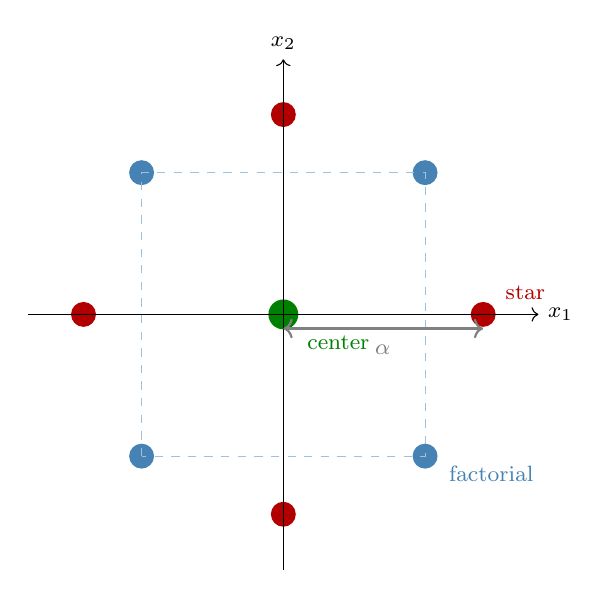
\begin{tikzpicture}[scale=1.8]
  % Factorial points
  \fill[steelblue] (-1,-1) circle (2.5pt);
  \fill[steelblue] (1,-1) circle (2.5pt);
  \fill[steelblue] (-1,1) circle (2.5pt);
  \fill[steelblue] (1,1) circle (2.5pt);

  % Star points
  \fill[red!70!black] (-1.41,0) circle (2.5pt);
  \fill[red!70!black] (1.41,0) circle (2.5pt);
  \fill[red!70!black] (0,-1.41) circle (2.5pt);
  \fill[red!70!black] (0,1.41) circle (2.5pt);

  % Center points
  \fill[green!50!black] (0,0) circle (3pt);

  % Axes
  \draw[->] (-1.8,0) -- (1.8,0) node[right] {\footnotesize $x_1$};
  \draw[->] (0,-1.8) -- (0,1.8) node[above] {\footnotesize $x_2$};

  % Labels
  \draw[dashed, steelblue!50] (-1,-1) rectangle (1,1);
  \node[below right, steelblue] at (1.1,-1) {\footnotesize factorial};
  \node[right, red!70!black] at (1.5,0.15) {\footnotesize star};
  \node[right, green!50!black] at (0.1,-0.2) {\footnotesize center};

  % Alpha annotation
  \draw[<->, thick, gray] (0,-0.1) -- (1.41,-0.1);
  \node[below, gray] at (0.7,-0.15) {\footnotesize $\alpha$};
\end{tikzpicture}
\captionof{figure}{Central Composite Design for 2 factors. Blue squares are
factorial points, red circles are star (axial) points, and the green circle is
the center point.}
\end{center}

The value of $\alpha$ determines the design's properties:
\begin{itemize}[nosep]
\item $\alpha = 1$: Face-centered CCD (star points on the face of the cube).
      Does not require runs outside the factor range, but the quadratic fit is
      less precise.
\item $\alpha = \sqrt{k}$: Spherical CCD. Star points lie on the sphere
      circumscribing the factorial cube.
\item $\alpha = (2^k)^{1/4}$: Rotatable CCD. The prediction variance is
      constant at all points equidistant from the center, making the model
      equally precise in all directions.
\end{itemize}

\subsection{Run Count}

\begin{center}
\begin{tabular}{ccccc}
\toprule
Factors & Factorial & Star & Center & Total \\
\midrule
2 & 4 & 4 & 5 & 13 \\
3 & 8 & 6 & 6 & 20 \\
4 & 16 & 8 & 7 & 31 \\
5 & 32 & 10 & 8 & 50 \\
\bottomrule
\end{tabular}
\end{center}

\subsection{Understanding Alpha}

The parameter $\alpha$ controls how far the star (axial) points extend beyond
the factorial cube. In plain language, it determines how ``extreme'' your
additional test conditions will be.

When $\alpha = 1$, the star points land exactly on the face of the cube. This
is called a \emph{face-centered} CCD. The star points test at the same extreme
values as the factorial points, just along one axis at a time. No run goes
beyond the original factor range, which is convenient when equipment or safety
limits constrain your experiments.

When $\alpha > 1$, the star points push beyond the cube into more extreme
territory. The rotatable value $\alpha = (2^k)^{1/4}$ (e.g., $\alpha = 1.41$
for $k = 2$ factors, $\alpha = 1.68$ for $k = 3$) ensures that the prediction
variance is the same at all points equidistant from the center. This improves
the quality of the quadratic fit but requires running experiments at conditions
outside the original factor range.

\medskip
\noindent\textbf{Practical example.}
Suppose temperature ranges from 150--200\textdegree C (center = 175\textdegree C,
half-range = 25\textdegree C). For a 2-factor CCD with $\alpha = 1.41$, the
star points along the temperature axis are at:
\[
175 \pm 1.41 \times 25 = 175 \pm 35.25
\]
This means testing at 139.75\textdegree C and 210.25\textdegree C. If your
equipment cannot reach these temperatures safely, use a face-centered design
($\alpha = 1$) instead, which keeps the star points at 150\textdegree C and
200\textdegree C. The face-centered design sacrifices some statistical
optimality (the quadratic terms are estimated less precisely), but it stays
within practical operating limits.

\section{Box--Behnken Design}

\begin{keypoint}[Box--Behnken Advantage]
Box--Behnken designs avoid extreme corners of the design space. Every run has
at most two factors at their extreme levels; the remaining factors are at the
center. This makes them safer for physical experiments where corner points are
dangerous or infeasible.
\end{keypoint}

\begin{center}
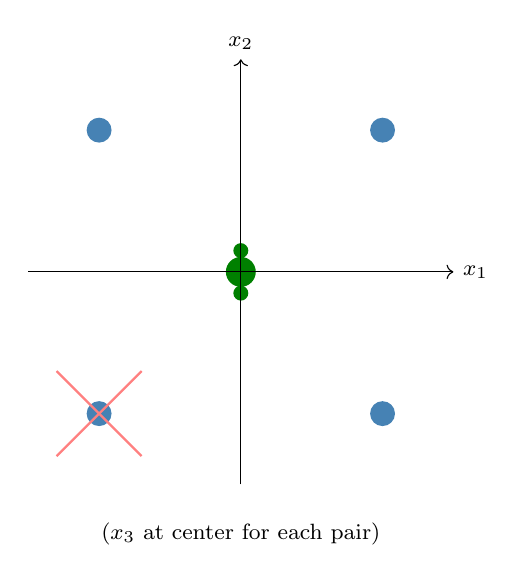
\begin{tikzpicture}[scale=1.8]
  % Edge midpoints for 2 factors (projected from 3D BB)
  \fill[steelblue] (-1,-1) circle (2.5pt);
  \fill[steelblue] (1,-1) circle (2.5pt);
  \fill[steelblue] (-1,1) circle (2.5pt);
  \fill[steelblue] (1,1) circle (2.5pt);

  % Missing corners (these would be dangerous)
  \draw[red!50, thick] (-1.3,-1.3) -- (-0.7,-0.7);
  \draw[red!50, thick] (-1.3,-0.7) -- (-0.7,-1.3);

  % Edge midpoints representing the 3rd factor at center
  \fill[green!50!black] (0,0) circle (3pt);
  \fill[green!50!black] (0,0.15) circle (1.5pt);
  \fill[green!50!black] (0,-0.15) circle (1.5pt);

  % Axes
  \draw[->] (-1.5,0) -- (1.5,0) node[right] {\footnotesize $x_1$};
  \draw[->] (0,-1.5) -- (0,1.5) node[above] {\footnotesize $x_2$};

  \node[below, font=\footnotesize] at (0,-1.7) {($x_3$ at center for each pair)};
\end{tikzpicture}
\captionof{figure}{Box--Behnken design concept. The extreme corner (crossed
out) is not tested. Each pair of factors is tested at all four edge
combinations while the third stays at center.}
\end{center}

For 3 factors, Box--Behnken requires 15 runs (12 edge-midpoint runs + 3 center
replicates), compared to 20 for a CCD. For 4 factors: 27 runs.

\subsection{When to Use Box--Behnken vs.\ CCD}

\begin{center}
\begin{tabular}{lcc}
\toprule
Criterion & CCD & Box--Behnken \\
\midrule
Avoids extreme corners & No & Yes \\
Points outside factor range & Yes (star) & No \\
Minimum factors & 2 & 3 \\
Sequential augmentation from $2^k$ & Yes & No \\
Rotatable option & Yes & No \\
Fewer runs (3--4 factors) & Depends & Often \\
\bottomrule
\end{tabular}
\end{center}

\subsection{Box--Behnken Worked Example}

Consider an experiment with 3 factors: temperature (150--200\textdegree C),
pressure (2--6 bar), and catalyst concentration (0.5--2.0 g/L). The coded
center values are 175\textdegree C, 4 bar, and 1.25 g/L respectively. The
complete 15-run Box--Behnken design matrix in actual (uncoded) values is:

\begin{center}
\begin{tabular}{cccc}
\toprule
Run & Temperature (\textdegree C) & Pressure (bar) & Catalyst (g/L) \\
\midrule
 1 & 150 & 2 & 1.25 \\
 2 & 200 & 2 & 1.25 \\
 3 & 150 & 6 & 1.25 \\
 4 & 200 & 6 & 1.25 \\
 5 & 150 & 4 & 0.5 \\
 6 & 200 & 4 & 0.5 \\
 7 & 150 & 4 & 2.0 \\
 8 & 200 & 4 & 2.0 \\
 9 & 175 & 2 & 0.5 \\
10 & 175 & 6 & 0.5 \\
11 & 175 & 2 & 2.0 \\
12 & 175 & 6 & 2.0 \\
13 & 175 & 4 & 1.25 \\
14 & 175 & 4 & 1.25 \\
15 & 175 & 4 & 1.25 \\
\bottomrule
\end{tabular}
\end{center}

Notice the structure: in runs 1--4, catalyst (factor C) is held at its center
value (1.25 g/L) while temperature and pressure vary at their extremes. In
runs 5--8, pressure (factor B) is at its center (4 bar) while temperature and
catalyst vary. In runs 9--12, temperature (factor A) is at its center
(175\textdegree C) while pressure and catalyst vary. Runs 13--15 are center
points where all three factors are at their midpoints.

Critically, no run has all three factors at their extreme levels
simultaneously. The corner point (200\textdegree C, 6 bar, 2.0 g/L) is never
tested---precisely the condition that might cause a dangerous runaway reaction.
This is the defining safety advantage of the Box--Behnken design.

\section{Latin Hypercube Sampling}

Latin Hypercube Sampling (LHS) is a space-filling design used primarily for
computer experiments and simulations where the response is deterministic (no
random error).

\subsection{Construction}

For $n$ samples and $k$ factors:
\begin{enumerate}[nosep]
\item Divide each factor's range into $n$ equal intervals.
\item Place exactly one sample point in each interval of each factor.
\item The placement within each interval is random.
\end{enumerate}

This guarantees that the projection onto any single factor axis covers the
entire range uniformly---a property called \emph{stratification}.

\subsection{When to Use LHS}

\begin{itemize}[nosep]
\item Computer experiments with deterministic outputs (no noise)
\item High-dimensional spaces (many factors) where factorial designs are infeasible
\item Building surrogate models (kriging, Gaussian processes)
\item Sensitivity analysis and uncertainty quantification
\end{itemize}


\section{Quick Reference: Choosing a Design}

\begin{center}
\begin{tabular}{lcccc}
\toprule
Design & Best For & Min Runs & Interactions? & Finds Optimum? \\
\midrule
Full Factorial & Complete picture & $2^k$ & All & No \\
Fractional Fact. & Screening + some 2FIs & $2^{k-p}$ & Some & No \\
Plackett--Burman & Fast screening & $k{+}1$ & No & No \\
Latin Hypercube & Exploration & Your choice & No & No \\
CCD & Finding the optimum & $2^k{+}2k{+}c$ & Yes & Yes \\
Box--Behnken & Safe optimization & $\sim 15$--$46$ & Yes & Yes \\
\bottomrule
\end{tabular}
\end{center}

\begin{keypoint}[The Decision Rule]
\textbf{2--4 factors, want everything:} Full Factorial.
\textbf{5+ factors, screening:} Plackett--Burman.
\textbf{2--5 factors, finding the optimum:} CCD (corners OK) or Box--Behnken
(avoid corners). \textbf{Computer simulation:} Latin Hypercube.
\end{keypoint}


% ═══════════════════════════════════════════
% PART III: ANALYSIS
% ═══════════════════════════════════════════
\part{Analysis and Optimization}

% ───────────────────────────────────────────
\chapter{Analyzing Results}
% ───────────────────────────────────────────

\section{The Pareto Chart}

The Pareto chart is the single most useful visualization in DOE. It displays
factors sorted by the absolute magnitude of their main effects, with a
cumulative percentage line overlaid.

\begin{keypoint}[The 80/20 Rule]
The Pareto principle states that roughly 80\% of the total effect magnitude is
caused by 20\% of the factors. The Pareto chart's cumulative line helps you
identify these ``vital few'' factors. Factors below the 80\% line are
candidates for being fixed at their cheapest or most convenient level.
\end{keypoint}

\subsection{Reading a Pareto Chart}

\begin{enumerate}[nosep]
\item Factors are sorted from largest to smallest absolute effect (top to bottom
      or left to right).
\item The bar length represents the magnitude of the main effect.
\item The cumulative line shows the running total as a percentage of the sum of
      all effect magnitudes.
\item The 80\% reference line marks where the ``vital few'' end and the
      ``trivial many'' begin.
\end{enumerate}

\section{Main Effects Plots}

A main effects plot shows the mean response at each level of a factor, connected
by line segments. The slope of the line indicates the magnitude and direction of
the effect.

\begin{itemize}[nosep]
\item A steep line means a large effect.
\item A flat line means the factor has little influence.
\item A non-linear pattern (for $>$2 levels) suggests curvature.
\end{itemize}

\section{Interaction Plots}

An interaction plot shows the mean response for each combination of two factors.
If the lines are parallel, there is no interaction. If they cross or diverge,
the interaction is significant.

\begin{keypoint}[How to Spot Interactions]
\textbf{Parallel lines} = no interaction (the effect of $A$ is the same
regardless of $B$'s level). \textbf{Non-parallel lines} = interaction.
\textbf{Crossing lines} = strong interaction (the best level of $A$ depends
on $B$'s level---this completely changes your recommendation).
\end{keypoint}

\section{Reading Tool Output}

When you run the analysis tool, the output looks like this:

\begin{lstlisting}[basicstyle=\footnotesize\ttfamily]
=== Main Effects: throughput ===
Factor             Effect  Std Error  % Contribution
------------------------------------------------------
buffer_pool_size  +850.3      45.2         62.1%
worker_threads    +312.7      45.2         22.8%
gc_heap_size      +142.1      45.2         10.4%
log_level          -64.5      45.2          4.7%
\end{lstlisting}

\noindent How to read each column:
\begin{itemize}[nosep]
\item \textbf{Effect:} How much the response changes when the factor goes from
      low to high. Positive means ``high level produces more.'' Negative means
      ``high level produces less.''
\item \textbf{Std Error:} The uncertainty in the effect estimate. Smaller is
      more precise. If the effect is much larger than its std error ($>$2--3$\times$),
      the effect is likely real, not noise.
\item \textbf{\% Contribution:} How much of the total variation this factor
      explains. The Pareto chart visualizes this. Factors totaling $\sim$80\%
      are the ``vital few.''
\end{itemize}

\begin{example}[Interpreting Confidence Intervals]
\begin{lstlisting}[basicstyle=\footnotesize\ttfamily]
temperature:  effect=+8.5, 95% CI=[+3.2, +13.8]
pressure:     effect=+1.2, 95% CI=[-4.1, +6.5]
\end{lstlisting}
\textbf{Temperature:} The CI is entirely positive, so the effect is
statistically significant. Temperature definitely matters.\\
\textbf{Pressure:} The CI includes zero, so the effect is NOT statistically
significant. The observed $+1.2$ could be noise.
\end{example}

\section{Complete Worked Example}

Let us walk through a full analysis of a $2^3$ factorial experiment, step by step,
with real numbers. Suppose we are studying the effect of three factors on the
response time (in milliseconds) of an API endpoint:

\begin{itemize}[nosep]
\item \textbf{A}: Cache enabled ($-1$ = off, $+1$ = on)
\item \textbf{B}: Thread pool size ($-1$ = 4 threads, $+1$ = 16 threads)
\item \textbf{C}: Compression ($-1$ = off, $+1$ = on)
\end{itemize}

\subsection{Step 1: The Raw Data}

\begin{center}
\begin{tabular}{cccccr}
\toprule
Run & $A$ & $B$ & $C$ & $AB$ & Response (ms) \\
\midrule
1 & $-1$ & $-1$ & $-1$ & $+1$ & 120 \\
2 & $+1$ & $-1$ & $-1$ & $-1$ & 75 \\
3 & $-1$ & $+1$ & $-1$ & $-1$ & 95 \\
4 & $+1$ & $+1$ & $-1$ & $+1$ & 40 \\
5 & $-1$ & $-1$ & $+1$ & $+1$ & 130 \\
6 & $+1$ & $-1$ & $+1$ & $-1$ & 82 \\
7 & $-1$ & $+1$ & $+1$ & $-1$ & 105 \\
8 & $+1$ & $+1$ & $+1$ & $+1$ & 48 \\
\bottomrule
\end{tabular}
\end{center}

The grand mean is $\bar{y} = (120+75+95+40+130+82+105+48)/8 = 86.875$ ms.

\subsection{Step 2: Calculate the Main Effect of A (Cache)}

Average response when $A = +1$ (cache on): $\bar{y}_{A+} = (75 + 40 + 82 + 48)/4 = 61.25$

Average response when $A = -1$ (cache off): $\bar{y}_{A-} = (120 + 95 + 130 + 105)/4 = 112.50$

\[
\text{ME}_A = \bar{y}_{A+} - \bar{y}_{A-} = 61.25 - 112.50 = -51.25 \text{ ms}
\]

The negative sign means cache \emph{reduces} response time (good!). Enabling the
cache cuts response time by an average of 51.25\,ms. The corresponding model
coefficient is $\text{ME}_A / 2 = -25.625$.

\subsection{Step 3: Calculate Main Effects of B and C}

By the same procedure:
\begin{align*}
\text{ME}_B &= \frac{95+40+105+48}{4} - \frac{120+75+130+82}{4} = 72.0 - 101.75 = -29.75 \text{ ms} \\
\text{ME}_C &= \frac{130+82+105+48}{4} - \frac{120+75+95+40}{4} = 91.25 - 82.50 = +8.75 \text{ ms}
\end{align*}

More threads (B) reduce response time by 29.75\,ms. Compression (C) actually
\emph{increases} response time by 8.75\,ms (the CPU cost of compression outweighs
the bandwidth savings).

\subsection{Step 4: Calculate the AB Interaction}

The $AB$ column is the element-wise product of the $A$ and $B$ columns. We compute:

$\bar{y}_{AB,\text{concordant}} = (120 + 40 + 130 + 48)/4 = 84.50$ (runs where $A$
and $B$ have the same sign)

$\bar{y}_{AB,\text{discordant}} = (75 + 95 + 82 + 105)/4 = 89.25$ (runs where $A$
and $B$ have opposite signs)

\[
\text{IE}_{AB} = 84.50 - 89.25 = -4.75 \text{ ms}
\]

This is a small interaction. The effect of cache does not depend strongly on the
thread pool size.

\subsection{Step 5: Pareto Ranking}

Ranking by absolute effect magnitude:

\begin{center}
\begin{tabular}{lrr}
\toprule
Factor & $|\text{Effect}|$ & Cumulative \% \\
\midrule
A (Cache) & 51.25 & 54.1\% \\
B (Threads) & 29.75 & 85.5\% \\
C (Compression) & 8.75 & 94.7\% \\
AB & 4.75 & 99.7\% \\
\bottomrule
\end{tabular}
\end{center}

Cache and thread pool size together account for 85.5\% of the total effect---these
are the ``vital few.'' Compression and the AB interaction are minor.

\subsection{Step 6: Confidence Intervals}

Suppose from replicated runs we estimated the pooled standard deviation as
$s = 6.0$\,ms. With $N = 8$ runs, the standard error of any main effect is:
\[
\text{SE} = \frac{2s}{\sqrt{N}} = \frac{2 \times 6.0}{\sqrt{8}} = 4.24 \text{ ms}
\]

For a 95\% confidence interval with, say, $\nu = 8$ degrees of freedom
($t_{0.025, 8} = 2.306$):

\begin{center}
\begin{tabular}{lrl}
\toprule
Factor & Effect & 95\% CI \\
\midrule
A (Cache) & $-51.25$ & $[-61.03, -41.47]$ \\
B (Threads) & $-29.75$ & $[-39.53, -19.97]$ \\
C (Compression) & $+8.75$ & $[-1.03, +18.53]$ \\
\bottomrule
\end{tabular}
\end{center}

\subsection{Step 7: Conclusions}

\begin{enumerate}[nosep]
\item \textbf{Cache (A)} is the dominant factor. Its CI is entirely negative
      (reduces response time). Enable the cache.
\item \textbf{Thread pool (B)} is the second most important factor. Its CI is
      entirely negative. Use 16 threads.
\item \textbf{Compression (C)} is not statistically significant---its CI
      includes zero. The 8.75\,ms increase could be noise. Leave compression off
      (it also saves CPU).
\item The \textbf{AB interaction} is small and not significant. Cache and threads
      help independently.
\item \textbf{Predicted best configuration}: Cache on, 16 threads, compression
      off. Predicted response: $86.875 - 25.625 - 14.875 - 4.375 = 42.0$\,ms.
      (This matches run~4 closely.)
\end{enumerate}


\section{Statistical Significance}

\subsection{Using Confidence Intervals}

For each main effect, compute the 95\% confidence interval:
\[
\text{CI} = \text{ME} \pm t_{0.025, \nu} \cdot \text{SE}
\]

If the interval does not contain zero, the effect is statistically significant.
Report the confidence interval alongside the point estimate---it conveys both
the magnitude and the uncertainty.

\subsection{Practical vs.\ Statistical Significance}

A factor can be statistically significant (the CI excludes zero) but practically
unimportant (the effect is tiny). Conversely, a factor can be practically
important but not statistically significant (the experiment was too small to
detect it). Always consider both.

\begin{warning}[Do Not Over-Rely on $p$-Values]
A $p$-value tells you how unlikely the observed data would be if the true effect
were zero. It does \emph{not} tell you the probability that the effect is real,
nor the magnitude of the effect. Focus on effect sizes and confidence intervals.
\end{warning}


% ───────────────────────────────────────────
\chapter{Response Surface Methodology}
% ───────────────────────────────────────────

\section{From Effects to Models}

Screening and factorial designs answer the question: ``Which factors matter?''
Response Surface Methodology (RSM) answers: ``What are the optimal settings?''

RSM fits a polynomial model to the data and uses the model to predict the
response at untested factor combinations, including the predicted optimum.

\section{What Is a Response Surface?}

Imagine your response is the elevation on a landscape. Each factor is a
direction you can walk---north-south, east-west. A \emph{linear model} says the
landscape is a flat tilted plane: walking north always goes uphill at the same
rate, no matter where you are. A \emph{quadratic model} allows hills and
valleys: there can be a peak (maximum) somewhere in the middle, and walking past
it starts going downhill.

Response Surface Methodology is about mapping this landscape with a minimum
number of measurements, then finding the highest peak (if you want to maximize)
or the lowest valley (if you want to minimize). Instead of measuring the
elevation at thousands of grid points, you strategically place a few dozen
measurement stations (your experimental runs) and fit a smooth mathematical
surface through them. The surface tells you not just what the response is
\emph{at} your measurement points, but predicts what it would be \emph{between}
them---including the location of the peak.

The power of RSM is that a quadratic model with $k$ factors requires only about
$2k^2$ measurements to fit, while a fine grid search would require hundreds or
thousands. With 3 factors and 20 well-placed runs, you can map a landscape that
a $10 \times 10 \times 10 = 1000$-point grid would struggle to reveal.

\section{Fitting the Model}

Given $n$ observations, the linear model in matrix form is:
\[
\mathbf{y} = \mathbf{X}\boldsymbol{\beta} + \boldsymbol{\epsilon}
\]

The least-squares estimate is:
\[
\hat{\boldsymbol{\beta}} = (\mathbf{X}^T\mathbf{X})^{-1}\mathbf{X}^T\mathbf{y}
\]

For a linear model with $k$ factors, $\mathbf{X}$ is an $n \times (k+1)$ matrix
(including the intercept column). For a quadratic model, $\mathbf{X}$ has
$1 + 2k + \binom{k}{2}$ columns (intercept + linear + squared + interaction
terms).

\subsection{A Concrete Fitting Example}

To see how the matrix equation works in practice, consider 5 data points from a
2-factor CCD (4 factorial corners plus 1 center point). We will fit a linear
model $Y = b_0 + b_1 x_1 + b_2 x_2$. The design matrix $\mathbf{X}$ (with
intercept column) and response vector $\mathbf{y}$ are:

\[
\mathbf{X} = \begin{pmatrix}
1 & -1 & -1 \\
1 & +1 & -1 \\
1 & -1 & +1 \\
1 & +1 & +1 \\
1 &  0 &  0
\end{pmatrix},
\qquad
\mathbf{y} = \begin{pmatrix}
61.1 \\ 77.7 \\ 66.9 \\ 84.3 \\ 72.5
\end{pmatrix}
\]

The least-squares solution minimizes the sum of squared residuals. In practice,
you do not compute this by hand---the tool does it automatically. But
understanding the structure helps you interpret the coefficients.

Applying $\hat{\boldsymbol{\beta}} = (\mathbf{X}^T\mathbf{X})^{-1}
\mathbf{X}^T\mathbf{y}$ yields:
\[
\hat{b}_0 = 72.5, \qquad \hat{b}_1 = +8.3, \qquad \hat{b}_2 = -3.1
\]

Interpreting each coefficient:
\begin{itemize}[nosep]
\item $b_0 = 72.5$ is the predicted response at the center of the design space.
\item $b_1 = +8.3$ means increasing factor $A$ by one coded unit increases the
      response by 8.3.
\item $b_2 = -3.1$ means increasing factor $B$ by one coded unit decreases the
      response by 3.1.
\end{itemize}

\section{Model Adequacy}

\subsection{$R^2$ and Adjusted $R^2$}

$R^2$ always increases when you add terms to the model, even if those terms are
pure noise. Adjusted $R^2$ penalizes for model complexity:

\begin{itemize}[nosep]
\item $R^2 > 0.9$: Excellent fit
\item $0.7 < R^2 < 0.9$: Good fit, some unexplained variation
\item $R^2 < 0.7$: Consider adding terms or transforming variables
\end{itemize}

A large gap between $R^2$ and $R^2_{\text{adj}}$ suggests overfitting.

\subsection{Residual Analysis}

Always check the residuals $e_i = y_i - \hat{y}_i$:
\begin{itemize}[nosep]
\item Plot residuals vs.\ fitted values: should show no pattern
\item Plot residuals vs.\ run order: should show no trend (drift)
\item Normal probability plot of residuals: should be approximately linear
\end{itemize}

\subsection{Interpreting Residual Plots}

Good residuals look like random scatter---no patterns, no trends, no funnels.
Here is what to look for and what each pattern means:

\begin{itemize}[nosep]
\item If residuals fan out (larger spread at higher fitted values), try a log
      transformation of the response.
\item If residuals show a curved pattern, add squared terms to the model.
\item If residuals trend with run order, there is drift in your experiment---blocking
      should have been used.
\end{itemize}

\begin{keypoint}[Residual Health Check]
Residual plots are your model's health check. Always look at them before
trusting any predictions.
\end{keypoint}

\section{Finding the Optimum}

For a quadratic model, the stationary point (where the partial derivatives are
zero) can be found analytically:
\[
\hat{\mathbf{x}}_s = -\frac{1}{2}\mathbf{B}^{-1}\mathbf{b}
\]
where $\mathbf{b}$ is the vector of linear coefficients and $\mathbf{B}$ is the
matrix of quadratic and interaction coefficients.

If the stationary point is a maximum (all eigenvalues of $\mathbf{B}$ are
negative), it is the predicted optimum for a ``maximize'' response. If it is a
minimum (all eigenvalues positive), it is the optimum for ``minimize.'' If
eigenvalues have mixed signs, the stationary point is a saddle point, and the
optimum lies on the boundary of the design space.

\begin{keypoint}[Confirmation Runs]
Never trust a predicted optimum without verification. Run 3--5 confirmation
experiments at the predicted settings. If the observed response matches the
prediction (within the confidence interval), the model is validated.
\end{keypoint}

\section{When the Optimum Is Outside Your Design Space}

Sometimes the stationary point computed from your quadratic model falls outside
the region you actually tested. For example, you tested temperature from 150 to
200\textdegree C, but the model predicts the optimum at 220\textdegree C. This
does \emph{not} mean you should blindly set temperature to 220\textdegree
C---the model is a polynomial approximation that may be wildly inaccurate
outside the tested range.

Instead, use the \textbf{method of steepest ascent} (or steepest descent, for
minimization):

\begin{enumerate}[nosep]
\item From your current factorial or RSM analysis, identify the direction of
      greatest improvement. This is determined by the linear coefficients of
      your model: the factor with the largest positive coefficient (for
      maximization) points in the most promising direction.
\item Starting from the center of your current design, take a series of steps
      along this direction. Each step increases (or decreases) each factor in
      proportion to its coefficient. For example, if the temperature coefficient
      is twice the pressure coefficient, increase temperature by 10 units for
      every 5 units of pressure increase.
\item Run a few experiments (3--5) along this path, spaced out enough to see
      the trend. The response will initially improve, then plateau or decline.
\item Center your next RSM design at the point where the response was best
      (just before it started declining). Run a new CCD or Box--Behnken there
      to find the precise optimum in that neighborhood.
\end{enumerate}

\begin{keypoint}[Steepest Ascent Is Iterative]
Think of steepest ascent as hiking uphill in fog. You cannot see the summit, but
you can feel which direction is steepest. You walk that way until the ground
levels off, then stop and survey the local area more carefully (a new RSM
design). You may need several rounds of ``hike, then survey'' to reach the true
summit.
\end{keypoint}


\section{Multi-Response Optimization}

When multiple responses must be optimized simultaneously (e.g., maximize yield
while minimizing cost), the \emph{desirability function} approach is standard:

\begin{enumerate}[nosep]
\item For each response $i$, define a desirability $d_i$ that maps the response
      to a $[0, 1]$ scale (0 = unacceptable, 1 = ideal).
\item Compute the overall desirability as the geometric mean:
      $D = (d_1 \cdot d_2 \cdot \ldots \cdot d_m)^{1/m}$
\item Find the factor settings that maximize $D$.
\end{enumerate}

\subsection{Worked Example: Desirability Calculation}

Suppose yield has a desirability of $0.9$ at a candidate point and cost has a
desirability of $0.7$. The overall desirability is:
\[
D = (0.9 \times 0.7)^{1/2} = (0.63)^{1/2} = 0.79
\]

\subsection{Constructing Individual Desirability Functions}

For a response you want to \textbf{maximize}:
\begin{itemize}[nosep]
\item $d = 0$ below the minimum acceptable value.
\item $d = 1$ at or above the target value.
\item $d$ increases linearly between the minimum and the target.
\end{itemize}

For a response you want to \textbf{minimize}:
\begin{itemize}[nosep]
\item $d = 1$ at or below the target value.
\item $d = 0$ above the maximum acceptable value.
\item $d$ decreases linearly between the target and the maximum.
\end{itemize}

The geometric mean ensures that if ANY response is unacceptable ($d_i = 0$),
the overall desirability is zero, regardless of how good the other responses
are. This is a strict veto property: a single failing response kills the
candidate point.


% ═══════════════════════════════════════════
% PART IV: PRACTICE
% ═══════════════════════════════════════════
\part{Practice}

% ───────────────────────────────────────────
\chapter{Planning Your First Experiment}
% ───────────────────────────────────────────

Before you choose a design type, select factor levels, or write a configuration
file, you need to answer several fundamental questions. Skipping this planning
step is the single most common reason experiments fail or produce useless
results. This chapter provides a systematic checklist and a worked example to
guide you through the process.

\section{The Pre-Experiment Checklist}

\begin{keypoint}[Before You Design Anything, Answer These Questions]
Work through this checklist in order. Do not proceed to design selection until
you have clear answers for every item.
\end{keypoint}

\subsection{1. What Am I Trying to Learn or Optimize?}

State your objective in one sentence. Be specific. Not ``make the system
faster'' but ``maximize throughput in requests per second under realistic load.''
Not ``understand the process'' but ``identify which 3 of these 12 factors have
the largest effect on yield.''

Your objective determines everything else:
\begin{itemize}[nosep]
\item \textbf{Screening} (``which factors matter?'') $\to$ Plackett--Burman or
      fractional factorial.
\item \textbf{Characterization} (``how do they interact?'') $\to$ full factorial.
\item \textbf{Optimization} (``what are the best settings?'') $\to$ CCD or
      Box--Behnken.
\end{itemize}

\subsection{2. What Factors Can I Control?}

List \emph{all} candidate factors, even ones you are unsure about. It is better
to screen a factor and discover it does not matter than to omit it and miss
something important. For each factor, note:
\begin{itemize}[nosep]
\item Is it continuous (temperature, pressure) or categorical (algorithm A vs.\ B)?
\item Can I set it precisely and reproducibly?
\item Are there any constraints (safety limits, hardware limits)?
\end{itemize}

\subsection{3. What Are Reasonable Low and High Levels?}

\begin{warning}[Do Not Pick Levels Too Close Together]
If your low and high levels are too similar, the effect will be smaller than the
noise and you will conclude (incorrectly) that the factor does not matter. A
good rule of thumb: the difference between levels should span a range you
believe could produce a noticeable change. If you are unsure, err on the side of
a wider range---you can always narrow it later.
\end{warning}

For each factor, choose levels that:
\begin{itemize}[nosep]
\item Are practically achievable (do not set temperature to 5000\textdegree C)
\item Span a range where you expect the response to change
\item Avoid known failure regions (the system crashes above 90\% CPU)
\item Are far enough apart to produce a detectable signal
\end{itemize}

\subsection{4. What Will I Measure?}

Define each response precisely, including:
\begin{itemize}[nosep]
\item \textbf{Name:} What you call it (throughput, yield, latency)
\item \textbf{Units:} req/sec, \%, milliseconds
\item \textbf{How measured:} Which tool, which metric, over what time window
\item \textbf{Direction:} Are you maximizing or minimizing?
\end{itemize}

Vague responses like ``performance'' are a recipe for confusion. ``p99 latency in
milliseconds, measured by wrk2 over a 60-second steady-state window'' is
unambiguous and reproducible.

\subsection{5. How Noisy Is My System?}

Run 5--10 identical experiments (same settings) and measure the response. The
standard deviation tells you the noise floor. This determines:
\begin{itemize}[nosep]
\item Whether you need replication (high noise $\to$ more replicates)
\item How far apart your factor levels need to be (the effect must exceed the
      noise)
\item Whether DOE is even the right approach (if the noise is so large that no
      effect can be detected, fix the measurement system first)
\end{itemize}

\subsection{6. How Many Runs Can I Afford?}

Be realistic about your budget in time, money, or compute. This constrains your
design choice:
\begin{itemize}[nosep]
\item \textbf{8--12 runs:} Screening designs (PB, fractional factorial)
\item \textbf{16--32 runs:} Full factorials on 4--5 factors
\item \textbf{15--50 runs:} Response surface designs (CCD, Box--Behnken)
\end{itemize}

It is always better to run a smaller, well-chosen design than a larger design
you cannot complete.

\subsection{7. Are There Nuisance Variables I Should Block On?}

Nuisance variables are things that affect the response but are not factors you
want to study---time of day, batch of raw material, which server you run on,
which operator performs the test. If you know a nuisance variable exists, use
blocking:
\begin{itemize}[nosep]
\item Assign each block a complete (or balanced) subset of the design
\item The block effect is estimated and removed from the error, giving you
      sharper estimates of the effects you care about
\end{itemize}


\section{Worked Example: Planning a Web Server Optimization}

Let us walk through the checklist for a concrete scenario.

\begin{example}[Planning Worksheet: Nginx Optimization]
\textbf{1. Objective:} Maximize requests per second (throughput) for a static
file workload served by Nginx, while keeping p99 latency below 50\,ms.

\textbf{2. Candidate factors:}
\begin{center}
\begin{tabular}{llcc}
\toprule
Factor & Type & Low & High \\
\midrule
\texttt{worker\_processes} & continuous & 2 & 16 \\
\texttt{worker\_connections} & continuous & 256 & 2048 \\
\texttt{sendfile} & categorical & off & on \\
\texttt{tcp\_nopush} & categorical & off & on \\
\texttt{keepalive\_timeout} & continuous & 5\,s & 65\,s \\
\texttt{gzip} & categorical & off & on \\
\bottomrule
\end{tabular}
\end{center}

\textbf{3. Level rationale:} Worker processes range from 2 (well below the 8-core
CPU) to 16 (double the cores). Worker connections span a 8$\times$ range. The
categorical factors are simply on/off toggles.

\textbf{4. Responses:}
\begin{itemize}[nosep]
\item Throughput: requests/sec, measured by \texttt{wrk} over 30\,s steady state,
      maximize.
\item p99 latency: milliseconds, measured by \texttt{wrk}, minimize (constraint:
      must stay below 50\,ms).
\end{itemize}

\textbf{5. Noise estimate:} Five identical runs at default settings gave
throughput values of 12,340, 12,510, 12,280, 12,450, and 12,390. Standard
deviation $\approx 90$ req/s (about 0.7\% of the mean). Noise is low; single
replicates may suffice for screening.

\textbf{6. Budget:} Each run takes about 2 minutes. We can afford up to 20 runs
in a single session.

\textbf{7. Blocking:} We will run everything on the same machine in one session,
so no blocking is needed. If we had to split across two days, we would block on
day.

\textbf{Decision:} Six factors, budget of 20 runs. A Plackett--Burman design
with 12 runs screens all six factors. That leaves 8 runs for a follow-up
factorial on the top 3 factors. Total: 20 runs.
\end{example}


\section{Common Pitfalls in Planning}

\begin{enumerate}
\item \textbf{Starting with optimization before screening.} If you have more
      than 4--5 factors, do not jump straight to a CCD. Screen first, then
      optimize the vital few.

\item \textbf{Forgetting to define the response precisely.} ``Performance''
      is not a response. ``Median throughput in req/s over a 60-second window
      after 10 seconds of warm-up'' is a response.

\item \textbf{Choosing levels based on convenience, not signal.} Levels of
      100\,MB and 110\,MB for a buffer size are probably too close. Levels of
      100\,MB and 1\,GB will produce a detectable effect.

\item \textbf{Ignoring nuisance variables.} If your results depend on time of
      day, server load, or network conditions, and you do not block on them,
      they inflate your error and hide real effects.

\item \textbf{Not estimating noise before designing.} Without a noise estimate,
      you cannot know how many replicates you need or whether your factor levels
      are far enough apart. Always do a few preliminary runs.

\item \textbf{Planning more runs than you can complete.} An incomplete design is
      often unanalyzable. It is better to run an 8-run PB to completion than to
      abandon a 32-run factorial halfway through.
\end{enumerate}


% ───────────────────────────────────────────
\chapter{The Sequential Experimentation Strategy}
% ───────────────────────────────────────────

\section{Phase 1: Screening}

\textbf{Goal:} Identify the vital few factors from a large list of candidates.

\textbf{Design:} Plackett--Burman or Resolution III fractional factorial.

\textbf{Runs:} 8--20 (regardless of how many factors you have).

\textbf{Analysis:} Pareto chart, main effects. Ignore interaction estimates (they
are confounded). Rank factors by absolute effect magnitude.

\textbf{Decision:} Select the top 3--5 factors for further study. Fix the rest
at their cheapest, easiest, or most robust level.

\medskip
\noindent\textbf{Worked Example.}
A chemical company suspects 15 process parameters affect product quality.
They run a Plackett--Burman design with 20 runs (PB(20)), which can test up
to 19 factors in a single experiment. The Pareto chart of absolute effects
reveals that temperature, catalyst\_concentration, and mixing\_speed account
for 83\% of the observed variation. The remaining 12 parameters contribute
only noise-level effects and are fixed at their current operating values for
all subsequent experiments.

\medskip
\noindent\textbf{Tips for fixing unimportant factors.}
Set unimportant factors at the level that is cheapest, most convenient, or
most robust. If a factor has a small positive effect (beneficial but not
statistically significant), set it to its high level---it helps a little and
costs nothing extra in experimentation. If a factor has zero effect, set it
to whatever minimizes cost or operational complexity. The key insight is that
``not statistically significant'' does not mean ``has no effect at all;''
it means the effect is too small to matter relative to the noise. Use this to
your advantage by choosing levels that are operationally favorable.

\section{Phase 2: Characterization}

\textbf{Goal:} Understand main effects \emph{and} interactions among the important
factors.

\textbf{Design:} Full factorial ($2^k$ with $k = 3$--5) or Resolution V
fractional factorial.

\textbf{Runs:} 8--32.

\textbf{Analysis:} Full ANOVA, interaction effects, confidence intervals. Check
for curvature by including center points---if the center-point mean differs
significantly from the average of the corner points, curvature exists.

\textbf{Decision:} If no curvature, the optimal settings are at the best corner.
If curvature exists, proceed to Phase 3.

\medskip
\noindent\textbf{Understanding center points.}
Add 3--5 center points to your factorial design. Center points are runs where
every factor is set to the midpoint of its range. Because a purely linear model
predicts that the center-point response equals the average of all corner-point
responses, any significant difference between the center-point mean and the
corner-point mean is direct evidence of curvature. If their average differs
significantly from the average of the corners, you have curvature and need
Phase~3. A simple $t$-test comparing the two averages is sufficient; many DOE
software packages report this automatically.

\medskip
\noindent\textbf{Worked Example (continued).}
Continuing the chemical company example, a $2^3$ full factorial on
temperature, catalyst\_concentration, and mixing\_speed is run with 8 corner
runs plus 4 center-point replicates, for a total of 12 runs. The ANOVA
reveals a strong temperature $\times$ catalyst interaction: high catalyst
concentration amplifies the effect of temperature on product quality. The
4 center points have an average response of 82.3, while the average of the
8 corner points is 76.1. This statistically significant difference
($p = 0.003$) confirms curvature in the temperature direction, so the
optimum lies somewhere inside the design space, not at a corner. Phase~3 is
needed.

\medskip
\noindent\textbf{What if there is no curvature?}
If center points match the corner average (i.e., the curvature test yields
$p > 0.05$), the system is well described by a linear-plus-interactions model.
The optimal settings are at the best corner combination identified by the
factorial analysis. You may skip Phase~3 entirely and proceed directly to
confirmation runs (Phase~4). This saves 15--50 runs and is a perfectly valid
outcome---not every system has curvature.

\section{Phase 3: Optimization}

\textbf{Goal:} Find the optimal factor settings within the design space.

\textbf{Design:} Central Composite Design or Box--Behnken.

\textbf{Runs:} 15--50 (depending on the number of factors).

\textbf{Analysis:} Fit a quadratic RSM model. Check $R^2$, residuals, and the
location of the stationary point.

\textbf{Decision:} Identify the predicted optimum. If it is within the design
space, proceed to confirmation. If it is on the boundary, consider shifting the
design space and running a new experiment.

\medskip
\noindent\textbf{Model fitting.}
A quadratic RSM model with $k$ factors has $1 + 2k + \binom{k}{2}$ parameters:
one intercept, $k$ linear terms, $k$ squared terms, and $\binom{k}{2}$
interaction terms. For 3 factors this is 10 parameters (1 intercept, 3 linear,
3 squared, 3 interaction). A Box--Behnken design with 15 runs provides enough
data to estimate all 10 parameters with 5 degrees of freedom left for error
estimation. A CCD with 20 runs for 3 factors provides even more error degrees
of freedom.

\medskip
\noindent\textbf{Worked Example (continued).}
The Box--Behnken design on temperature, catalyst\_concentration, and
mixing\_speed (15 runs) reveals that temperature has a strong quadratic effect
with an optimum near 185\textdegree C---not at either extreme of the
150--200\textdegree C range. Catalyst concentration shows a linear increasing
trend: higher is better, at least within the tested range. The temperature
$\times$ catalyst interaction is significant, meaning that higher catalyst
concentration shifts the optimal temperature upward (from about 180\textdegree C
at low catalyst to 190\textdegree C at high catalyst). Mixing speed has a
moderate linear effect but no significant curvature or interactions.

\medskip
\noindent\textbf{Interpreting $R^2$.}
The coefficient of determination $R^2$ measures how much of the response
variation the model explains. If $R^2 > 0.85$, the model is adequate for
optimization---it captures the main trends and the predicted optimum is
likely reliable. If $R^2 < 0.7$, the model may be missing important terms or
there may be outliers distorting the fit. In this case, check the residual
plots for patterns, consider adding higher-order terms or transforming the
response, and inspect individual runs for measurement errors. Also check
$R^2_{\text{adj}}$, which penalizes for unnecessary terms: a large gap between
$R^2$ and $R^2_{\text{adj}}$ suggests overfitting.

\section{Phase 4: Confirmation}

\textbf{Goal:} Validate the predicted optimum.

\textbf{Design:} 3--5 replicate runs at the predicted optimal settings.

\textbf{Analysis:} Compare the observed mean to the predicted value. If the
observed value falls within the prediction interval, the model is confirmed.

\medskip
\noindent\textbf{How many confirmation runs?}
Run at least 3 independent replicates at the predicted optimum. Five replicates
are better if the measurement has high variability. Each replicate must be a
fully independent run---reset the equipment, prepare fresh materials, and
re-measure from scratch. Do not simply repeat the measurement on the same
batch, as that only estimates measurement error, not process variability.

\medskip
\noindent\textbf{What to compare.}
Compute the mean and confidence interval of the confirmation runs. If the
predicted value from the RSM model falls within this confidence interval, the
model is validated. Alternatively, compute a prediction interval from the model
(which accounts for both model uncertainty and noise) and check whether the
confirmation mean falls within it. Either approach works; the key is that the
predicted and observed values agree within statistical uncertainty.

\medskip
\noindent\textbf{What if it does not match?}
If the confirmation results are significantly different from the prediction,
the model may be over-fitted, the process may have drifted between the
optimization experiment and the confirmation runs, or the design space may
have shifted due to an uncontrolled variable (e.g., a new batch of raw
material). In this case, consider re-running Phase~3 with the design centered
on the confirmation results rather than the original center. This ``move and
re-fit'' strategy often converges in one additional round.

\section{Cost--Benefit Analysis of the Sequential Strategy}

The sequential approach is dramatically more efficient than brute-force
alternatives. Consider the chemical company example:

\begin{center}
\begin{tabular}{llr}
\toprule
Phase & Purpose & Runs \\
\midrule
Phase 1: Screening & PB(20) to screen 15 factors & 20 \\
Phase 2: Characterization & $2^3$ + 4 center points on 3 factors & 12 \\
Phase 3: Optimization & Box--Behnken on 3 factors & 15 \\
Phase 4: Confirmation & Replicates at the predicted optimum & 5 \\
\midrule
\textbf{Total} & \textbf{From 15 unknowns to validated optimum} & \textbf{52} \\
\bottomrule
\end{tabular}
\end{center}

\noindent Compare this to the alternatives:

\begin{itemize}[nosep]
\item \textbf{Brute-force grid search} at 3 levels per factor:
      $3^{15} = 14{,}348{,}907$ runs. Even testing one combination per second
      would take over 166 days of continuous operation.
\item \textbf{Random search} would need hundreds of runs with no guarantee of
      finding the optimum. With 15 factors, even 500 random runs cover a
      vanishingly small fraction of the design space, and the results provide
      no structured information about interactions or curvature.
\item \textbf{One-variable-at-a-time (OVAT)} would require roughly
      $15 \times 3 = 45$ runs for initial screening, then more for each
      subsequent factor---but would miss all interactions and likely converge
      to a suboptimal solution.
\end{itemize}

\noindent The sequential DOE strategy achieves in 52 runs what grid search
attempts in 14 million: a validated, interaction-aware optimum with
quantified uncertainty.


% ───────────────────────────────────────────
\chapter{Applications}
% ───────────────────────────────────────────

\section{Software Performance Benchmarking}

Software systems have many tunable parameters---thread pool sizes, buffer
capacities, timeout values, caching strategies---and engineers often tune them
by intuition, one at a time. DOE provides a systematic alternative.

\subsection{Example: Database Configuration}

A database administrator suspects five configuration knobs affect transaction
throughput:

\begin{center}
\begin{tabular}{lcc}
\toprule
Factor & Low & High \\
\midrule
\texttt{buffer\_pool\_size} & 1\,GB & 4\,GB \\
\texttt{io\_capacity} & 200 & 2000 \\
\texttt{max\_connections} & 100 & 500 \\
\texttt{query\_cache} & 0\,MB & 256\,MB \\
\texttt{thread\_pool\_size} & 4 & 16 \\
\bottomrule
\end{tabular}
\end{center}

\textbf{Phase 1:} A Plackett--Burman design with 8 runs reveals that
\texttt{buffer\_pool\_size} and \texttt{io\_capacity} account for 75\% of the
throughput variation. The other three knobs have negligible effects.

\textbf{Phase 2:} A $2^2$ full factorial on the two important knobs (4 runs,
with 2 center points) confirms a significant interaction: large buffer pools
only help when I/O capacity is also high.

\textbf{Phase 3:} A CCD with 13 runs on the two knobs finds the optimal
settings: \texttt{buffer\_pool\_size} = 3.2\,GB, \texttt{io\_capacity} = 1600.

Total: 27 runs. An OVAT approach would have tested each knob at 3--4 values
($\approx$15--20 runs) and missed the interaction entirely.

\subsection{Example: Compiler Flags}

A performance engineer wants to understand how compiler optimization level
(\texttt{-O1}, \texttt{-O2}, \texttt{-O3}), link-time optimization
(\texttt{off}, \texttt{thin}, \texttt{full}), and architecture target
(\texttt{native}, \texttt{x86-64-v3}) affect runtime and binary size.

A $3 \times 3 \times 2 = 18$ full factorial tests all combinations. The analysis
reveals that \texttt{-O3} with \texttt{thin} LTO produces the best runtime, but
\texttt{full} LTO produces the smallest binary. The interaction between
optimization level and LTO is significant: \texttt{full} LTO improves
\texttt{-O1} more than \texttt{-O3} (diminishing returns when the optimizer has
already done most of the work).

\section{Scientific and Engineering Experiments}

\subsection{Example: Chemical Reactor Optimization}

A chemical engineer wants to maximize yield and purity while minimizing cost in a
batch reactor. Three factors are controlled: temperature (150--200\textdegree C),
pressure (2--6 bar), and catalyst concentration (0.5--2.0 g/L).

Running the reactor at all extremes simultaneously (200\textdegree C, 6 bar,
2.0 g/L) risks a runaway reaction. A Box--Behnken design avoids this: each run
has at most two factors at their extremes while the third is at center.

With 15 runs, the engineer fits a quadratic model for each response and discovers
that:
\begin{itemize}[nosep]
\item Temperature has the largest effect on yield (quadratic, with a maximum near
      185\textdegree C).
\item Catalyst concentration has the largest effect on purity (linear, higher is
      better).
\item Cost increases linearly with all three factors, with a temperature--pressure
      interaction.
\end{itemize}

The desirability function approach finds the compromise: 185\textdegree C,
3.5 bar, 1.8 g/L, yielding 78\% yield, 95\% purity, at \$55/batch.

\subsection{Lessons from the Reactor Example}

This example illustrates the central trade-off in multi-response optimization.
No single set of factor settings simultaneously maximizes yield, maximizes
purity, AND minimizes cost. The engineer must decide which response matters
most---or find a compromise using desirability functions.

The sequential strategy was crucial here: screening with Plackett--Burman would
have been wasted because there were only 3 factors. Starting directly with
Box--Behnken was the right call.

The quadratic effects (especially temperature's optimum at 185\textdegree C,
not at either extreme) could never have been detected by a 2-level factorial.
Response surface designs earn their keep precisely in these situations---when
the optimal setting lies between the extremes, not at them.

\subsection{Example: Materials Science}

A materials scientist studies the tensile strength of a new alloy as a function
of four processing parameters. A CCD with 31 runs reveals that annealing
temperature has a strong quadratic effect (optimum at 520\textdegree C) and
interacts with cooling rate. The quadratic model achieves $R^2 = 0.94$ and
correctly predicts the confirmation runs within $\pm 3\%$.

\subsection{Example: Microservice Configuration}

A platform team needs to optimize a Kubernetes-deployed microservice for latency
and cost. The controllable factors are:

\begin{center}
\begin{tabular}{lcc}
\toprule
Factor & Low & High \\
\midrule
\texttt{replicas} & 2 & 8 \\
\texttt{cpu\_limit} & 500m & 2 cores \\
\texttt{memory\_limit} & 512\,Mi & 2\,Gi \\
\texttt{hpa\_target\_cpu} & 50\% & 80\% \\
\bottomrule
\end{tabular}
\end{center}

A $2^4 = 16$ full factorial gives the complete picture. The analysis reveals
that more replicas only help up to a point (interaction with CPU limit), and
that doubling memory has no effect when CPU is the bottleneck. The team sets
\texttt{replicas=4}, \texttt{cpu\_limit=1.5}, \texttt{memory\_limit=512Mi},
\texttt{hpa\_target\_cpu=60\%}---saving 40\% on compute cost with no latency
increase.

\section{Machine Learning Hyperparameter Tuning}

DOE can replace random search or grid search for hyperparameter optimization.
The efficiency gains are dramatic:

\begin{center}
\begin{tabular}{lcl}
\toprule
Approach & Runs (8 params) & What You Learn \\
\midrule
Grid search ($3^8$) & 6,561 & Everything, wastefully \\
Random search & $\sim$100 & Noisy, unstructured \\
PB screening & 12 & Which 3 params matter \\
\quad + full factorial & 8 more & Their interactions \\
\textbf{Total DOE} & \textbf{20} & \textbf{Focused, actionable} \\
\bottomrule
\end{tabular}
\end{center}

\begin{itemize}[nosep]
\item \textbf{Screening:} Use a PB design to test 10+ hyperparameters and
      identify the 3--4 that actually affect validation accuracy.
\item \textbf{Optimization:} Use a CCD or LHS on the important hyperparameters
      to find the optimal region.
\item \textbf{Advantage over grid search:} A $2^{10}$ grid search requires
      1024 training runs. A PB screen requires 12.
\item \textbf{Advantage over random search:} LHS guarantees better space coverage
      than pure random sampling with the same number of points.
\end{itemize}

\begin{example}[Hyperparameter Screening in Practice]
A data scientist tests 8 hyperparameters (learning rate, batch size, dropout,
hidden layers, hidden units, optimizer, weight decay, activation) using a PB
design with 12 training runs. The Pareto chart immediately shows that
\texttt{learning\_rate}, \texttt{batch\_size}, and \texttt{hidden\_units}
account for 85\% of the validation accuracy variation. The other 5 parameters
are fixed at defaults, and a $2^3$ factorial (8 runs) on the important three
reveals that \texttt{learning\_rate} and \texttt{batch\_size} interact strongly.
Total: 20 training runs instead of 6,561.
\end{example}


% ───────────────────────────────────────────
\chapter{Common Mistakes and How to Avoid Them}
% ───────────────────────────────────────────

Even experienced experimenters fall into these traps. Each one can invalidate
your results or waste your budget. Learn them once, avoid them forever.

\section{Choosing Factor Levels Too Close Together}

\textbf{The mistake:} Testing temperature at 198\textdegree C and
202\textdegree C. The true effect is tiny relative to experimental noise, so
you conclude (incorrectly) that temperature does not matter.

\textbf{The fix:} Make the difference between levels large enough to produce a
detectable effect. A rule of thumb: the difference should be at least 2--3 times
the expected noise level. If your measurement varies by $\pm 5$\%, a 1\% change
in the factor level will be invisible.

\section{Not Randomizing Run Order}

\textbf{The mistake:} Running all ``high temperature'' experiments in the
morning and all ``low temperature'' experiments in the afternoon. Equipment
drift, ambient temperature changes, or operator fatigue get confounded with
your factor.

\textbf{The fix:} Always randomize. Use the \texttt{-{}-seed} flag for
reproducibility. Never run experiments in the order they appear in the design
matrix.

\section{Changing Other Things Between Runs}

\textbf{The mistake:} Updating the OS halfway through the experiment, or a
colleague restarting the server. Now some runs operated under different
conditions, and you cannot tell whether observed differences are due to your
factors or the environment change.

\textbf{The fix:} Keep everything constant except the factors you are studying.
If something does change unavoidably, use blocking to account for it---assign
a new block at the change point.

\section{Testing Too Many Factors Without Screening}

\textbf{The mistake:} Running a full factorial on 8 factors (256 runs) when only
3 of them matter. You burn 253 runs on factors that contribute nothing.

\textbf{The fix:} Start with a Plackett--Burman screening design (12 runs for
up to 11 factors). Identify the vital few, then focus your runs on those.

\section{Ignoring Interactions}

\textbf{The mistake:} You find that ``thread count = 32'' is best based on its
main effect. But in reality it is only best when combined with a large
connection pool. At a small connection pool, 32 threads actually makes things
worse (thread contention).

\textbf{The fix:} Use a design that estimates interactions (full factorial or
fractional factorial with Resolution IV+). Always check the interaction effects
table, not just main effects.

\section{Not Running Confirmation Experiments}

\textbf{The mistake:} Trusting the RSM model's predicted optimum without
verifying it. The model is a polynomial approximation---it may be wrong,
especially if you are near the edge of the design space.

\textbf{The fix:} Always run 3--5 experiments at the predicted optimal settings.
If the observed response matches the prediction (within the confidence interval),
you are done. If not, the model needs refinement.

\section{Confusing Replication with Repetition}

\textbf{The mistake:} Running the benchmark 5 times without restarting the
server and computing a standard deviation. This measures only \emph{measurement}
variability, not the full experimental variability that includes setup,
configuration application, and environmental factors.

\textbf{The fix:} True replication means independently resetting the entire
experimental setup between runs---restart the server, re-apply the
configuration, let it warm up, then measure. Use \texttt{block\_count > 1} to
get genuine replicates.

\begin{center}
\begin{tabular}{lll}
\toprule
 & Replication & Repetition \\
\midrule
What & Re-do entire setup & Re-measure same setup \\
Captures & Full experimental error & Measurement noise only \\
Example & Restart server, re-run & Run benchmark 3$\times$ \\
Use for & Estimating real variability & Estimating measurement noise \\
\bottomrule
\end{tabular}
\end{center}

\section{Over-Engineering the First Experiment}

\textbf{The mistake:} Spending weeks designing a 50-run CCD as your very first
experiment on a system you have never studied before.

\textbf{The fix:} Follow the sequential strategy. Your first experiment should
be a cheap screening design (8--12 runs). Learn which factors matter, then
invest runs wisely. You can always add more runs later; you cannot un-waste runs
you already spent.


% ───────────────────────────────────────────
\chapter{Using the DOE Helper Tool}
% ───────────────────────────────────────────

\section{Installation}

\begin{lstlisting}[language=bash]
# Clone the repository
git clone <repository-url>
cd design_of_experiments

# Install dependencies
pip install -r requirements.txt

# Or install as a package
pip install -e .
\end{lstlisting}

\section{Configuration File}

The tool is driven by a JSON configuration file:

\begin{lstlisting}[language=json]
{
  "metadata": {
    "name": "My Experiment",
    "description": "What I am investigating"
  },
  "factors": [
    {"name": "temperature", "levels": ["150", "200"],
     "type": "continuous", "unit": "C"},
    {"name": "catalyst", "levels": ["A", "B"],
     "type": "categorical"}
  ],
  "responses": [
    {"name": "yield", "optimize": "maximize", "unit": "%"},
    {"name": "cost",  "optimize": "minimize", "unit": "USD"}
  ],
  "settings": {
    "operation": "full_factorial",
    "test_script": "my_test.sh",
    "out_directory": "results",
    "block_count": 1
  }
}
\end{lstlisting}

\section{Configuration Reference}

This section documents every field in the JSON configuration file.

\subsection{Metadata Fields}

\begin{center}
\begin{tabular}{llp{5.5cm}}
\toprule
Field & Required & Description \\
\midrule
\texttt{name} & Yes & A short name for the experiment. Used in report titles and file names. \\
\texttt{description} & No & A longer description of the experiment's purpose. Appears in the HTML report header. \\
\bottomrule
\end{tabular}
\end{center}

\subsection{Factor Fields}

Each entry in the \texttt{factors} array describes one controllable input variable.

\begin{center}
\begin{tabular}{llp{5.5cm}}
\toprule
Field & Required & Description \\
\midrule
\texttt{name} & Yes & Identifier for the factor. Used as the column header and command-line argument name. Must be a valid identifier (letters, digits, underscores). \\
\texttt{levels} & Yes & Array of level values (as strings). For 2-level designs, provide exactly 2 values. For multi-level designs, provide all values. \\
\texttt{type} & No & \texttt{"continuous"} (default) or \texttt{"categorical"}. Continuous factors are coded to $[-1, +1]$ for analysis. Categorical factors are compared by level means. \\
\texttt{unit} & No & Unit of measurement (e.g., \texttt{"MB"}, \texttt{"ms"}, \texttt{"C"}). Displayed in reports and plots. \\
\texttt{description} & No & Human-readable description. Shown in the HTML report. \\
\bottomrule
\end{tabular}
\end{center}

\subsection{Response Fields}

Each entry in the \texttt{responses} array describes one measurable output.

\begin{center}
\begin{tabular}{llp{5.5cm}}
\toprule
Field & Required & Description \\
\midrule
\texttt{name} & Yes & Identifier for the response. Must match a key in the JSON output of your test script. \\
\texttt{optimize} & No & \texttt{"maximize"} (default) or \texttt{"minimize"}. Determines the direction of optimization in RSM analysis. \\
\texttt{unit} & No & Unit of measurement (e.g., \texttt{"req/s"}, \texttt{"\%"}). Displayed in reports. \\
\texttt{description} & No & Human-readable description of what is measured. \\
\bottomrule
\end{tabular}
\end{center}

\subsection{Runner Fields}

The \texttt{runner} section controls how factor values are passed to your test script.

\begin{center}
\begin{tabular}{llp{5.5cm}}
\toprule
Field & Required & Description \\
\midrule
\texttt{arg\_style} & No & How factor values are passed to the test script. Options below. Default: \texttt{"double-dash"}. \\
\bottomrule
\end{tabular}
\end{center}

\noindent The three argument styles:

\begin{description}[style=nextline, leftmargin=2.5cm]
\item[\texttt{double-dash}] Factors are passed as \texttt{-{}-factor\_name value}.
      Example: \texttt{./test.sh -{}-temperature 200 -{}-pressure 6}. This is the
      most common and explicit style.
\item[\texttt{env}] Factors are set as environment variables before invoking the
      script. Example: \texttt{temperature=200 pressure=6 ./test.sh}. Useful when
      your test script reads from the environment.
\item[\texttt{positional}] Factors are passed as positional arguments in the order
      they appear in the \texttt{factors} array. Example:
      \texttt{./test.sh 200 6}. Compact but fragile---reordering factors in the
      config will change which value goes where.
\end{description}

\subsection{Settings Fields}

\begin{center}
\begin{tabular}{llp{5.5cm}}
\toprule
Field & Required & Description \\
\midrule
\texttt{operation} & Yes & Design type. One of: \texttt{full\_factorial}, \texttt{fractional\_factorial}, \texttt{plackett\_burman}, \texttt{latin\_hypercube}, \texttt{central\_composite}, \texttt{box\_behnken}. \\
\texttt{test\_script} & Yes & Path to the executable that runs one experiment. Receives factor values and writes a JSON result file. \\
\texttt{block\_count} & No & Number of complete replicates of the entire design. Default: 1 (no replication). Set to 2 or 3 for noisy systems. \\
\texttt{out\_directory} & No & Directory where raw result JSON files are written. Default: \texttt{"results"}. \\
\texttt{processed\_directory} & No & Directory where analysis outputs (plots, CSV, reports) are saved. Default: \texttt{"processed"}. \\
\texttt{lhs\_samples} & No & Number of sample points for Latin Hypercube designs. Only used when \texttt{operation} is \texttt{latin\_hypercube}. Default: 20. \\
\bottomrule
\end{tabular}
\end{center}

\subsection{Fixed Factors}

The optional \texttt{fixed\_factors} object contains key-value pairs that are
passed to every run of the test script but are not varied in the design. Use
these for parameters that must be set but are not part of the experiment:

\begin{lstlisting}[language=json]
"fixed_factors": {
  "workload": "oltp_read_write",
  "duration": "60",
  "warmup": "10"
}
\end{lstlisting}

Fixed factors appear in the runner script as additional arguments (using the
same \texttt{arg\_style} as the experimental factors) and are recorded in the
report for reproducibility.


\section{Supported Operations}

\begin{center}
\begin{tabular}{lll}
\toprule
Operation & Design Type & Requirements \\
\midrule
\texttt{full\_factorial} & All combinations & Any levels \\
\texttt{fractional\_factorial} & $2^{k-p}$ fraction & 2 levels \\
\texttt{plackett\_burman} & PB screening & 2 levels \\
\texttt{latin\_hypercube} & Space-filling & Any \\
\texttt{central\_composite} & CCD & 2 numeric levels \\
\texttt{box\_behnken} & Box--Behnken & 2 numeric, $\geq$3 factors \\
\bottomrule
\end{tabular}
\end{center}

\section{Workflow}

\begin{lstlisting}[language=bash]
# 1. Preview the design
doe info --config config.json

# 2. Generate runner script
doe generate --config config.json --output run.sh --seed 42

# 3. Execute experiments
bash run.sh

# 4. Analyze results
doe analyze --config config.json

# 5. Get optimization recommendations
doe optimize --config config.json

# 6. Generate HTML report
doe report --config config.json --output report.html

# 7. Export to CSV
doe analyze --config config.json --csv results/csv
\end{lstlisting}

\section{Test Script Protocol}

Your test script must:
\begin{enumerate}[nosep]
\item Accept factor values via the configured argument style
      (\texttt{-{}-name value}, environment variables, or positional arguments).
\item Accept \texttt{-{}-out <path>} to specify the output file.
\item Write a JSON file to the output path with keys matching your response names.
\end{enumerate}

\begin{lstlisting}[language=bash]
#!/bin/bash
# Example test script
# ... run your experiment here ...
echo '{"yield": 85.3, "cost": 12.50}' > "$OUT_PATH"
\end{lstlisting}

\section{Analysis Output}

The \texttt{analyze} command computes and displays:
\begin{itemize}[nosep]
\item Main effects with standard errors and 95\% confidence intervals
\item Two-factor interaction effects (for 2-level factors)
\item Summary statistics (count, mean, std, min, max) per factor per level
\item Pareto chart with cumulative contribution line
\item Main effects plots (grid of line plots, one per factor)
\end{itemize}

The \texttt{optimize} command additionally fits a linear RSM model and reports
$R^2$, coefficients, predicted optimum, and factor importance ranking.

The \texttt{report} command generates a self-contained HTML file with all tables,
plots (embedded as base64 images), and a collapsible design matrix.


\section{Troubleshooting}

This section covers the most common problems users encounter and how to resolve
them.

\subsection{``My Effects Are All Near Zero''}

\textbf{Likely causes:}
\begin{itemize}[nosep]
\item Factor levels are too close together. If you test buffer size at 100\,MB
      and 110\,MB, the 10\% difference may be invisible against the noise. Widen
      your levels.
\item The response is dominated by noise. If the run-to-run variability is
      larger than any factor effect, nothing will be significant. Reduce noise
      (longer measurement windows, more stable environment) or increase
      replication.
\item You are studying the wrong factors. The real drivers of performance may
      not be in your factor list. Revisit your candidate list and consider
      factors you dismissed.
\end{itemize}

\subsection{``$R^2$ Is Very Low''}

An $R^2$ below 0.5 means the model explains less than half the variation.
\textbf{Likely causes:}
\begin{itemize}[nosep]
\item Important factors are missing from the model. There may be a factor you
      did not include that has a large effect.
\item The wrong model type is fitted. A linear model cannot capture curvature.
      If the true relationship is quadratic, try a response surface model.
\item The system is inherently very noisy, and single replicates are
      insufficient. Add replication to bring down the error variance.
\end{itemize}

\subsection{``Confidence Intervals Are Huge''}

Wide confidence intervals mean the effect estimates are imprecise.
\textbf{Likely causes:}
\begin{itemize}[nosep]
\item Not enough replication. With a single replicate of a $2^k$ design, the
      error variance is estimated from higher-order interactions (which may
      themselves be real effects). Adding even one replicate (\texttt{block\_count
      = 2}) dramatically improves precision.
\item High inherent noise. Reduce variability by controlling nuisance variables,
      using blocking, or increasing measurement duration.
\end{itemize}

\subsection{``The Predicted Optimum Is Unrealistic''}

If the RSM model predicts an optimum at factor settings that are physically
impossible or far outside your tested range:
\begin{itemize}[nosep]
\item The model is extrapolating beyond the design space. Polynomial models can
      produce absurd predictions outside the region where data exists. Never
      trust predictions more than 10--20\% beyond your tested range.
\item The stationary point is a saddle point, not a true optimum. Check the
      eigenvalues. If they have mixed signs, the optimum is on the boundary of
      the design space, not at the stationary point.
\item Consider shifting your design space toward the predicted optimum using
      steepest ascent (see Section on ``When the Optimum Is Outside Your Design
      Space'') and running a new experiment there.
\end{itemize}

\subsection{``Runner Script Fails on Some Runs''}

If some experimental runs succeed and others fail:
\begin{itemize}[nosep]
\item Check the test script's error handling. Does it handle edge cases at
      extreme factor combinations? A setting that works at (low, low) might
      crash at (high, high).
\item Look for missing result files. The analysis tool expects a JSON result
      file for every run. Missing files produce incomplete data that can bias
      the analysis.
\item Check disk space and permissions in the output directory.
\item Verify that the test script correctly parses all argument styles. A
      common bug: the script reads \texttt{-{}-factor\_name} but the config
      uses \texttt{env} style.
\item If only a few runs failed, you may still be able to analyze the partial
      results, but the design will no longer be balanced. The effect estimates
      will have unequal precision, and some interactions may not be estimable.
\end{itemize}


% ═══════════════════════════════════════════
% APPENDICES
% ═══════════════════════════════════════════
\appendix

\chapter{Mathematical Reference}

\section{Effect Estimation Formulas}

For a $2^k$ factorial with $N = 2^k$ runs, coded levels $x \in \{-1, +1\}$, and
response vector $\mathbf{y}$:

\paragraph{Main effect of factor $i$:}
\[
\text{ME}_i = \frac{2}{N} \sum_{j=1}^{N} x_{ij} y_j
= \bar{y}_{i+} - \bar{y}_{i-}
\]

\paragraph{Interaction effect of factors $i$ and $k$:}
\[
\text{IE}_{ik} = \frac{2}{N} \sum_{j=1}^{N} x_{ij} x_{kj} y_j
\]

\paragraph{Standard error of any effect:}
\[
\text{SE} = \frac{2s}{\sqrt{N}}
\]
where $s^2 = \text{MS}_E$ (mean square error from ANOVA or from replicates).

\paragraph{Sum of squares for any effect:}
\[
\text{SS}_{\text{effect}} = \frac{N}{4} \cdot \text{ME}^2
\]

\section{Response Surface Model}

For $k$ factors, the full quadratic model has $p = 1 + 2k + \binom{k}{2}$
parameters:
\[
\hat{y} = b_0 + \sum_{i=1}^k b_i x_i
+ \sum_{i=1}^k b_{ii} x_i^2
+ \sum_{i<j} b_{ij} x_i x_j
\]

\begin{center}
\begin{tabular}{cc}
\toprule
$k$ & $p$ (parameters) \\
\midrule
2 & 6 \\
3 & 10 \\
4 & 15 \\
5 & 21 \\
\bottomrule
\end{tabular}
\end{center}

The design must have at least $p$ distinct runs (and preferably $\geq 1.5p$) to
fit the model.

\section{Minimum Run Counts by Design}

\begin{center}
\begin{tabular}{lcccccc}
\toprule
 & \multicolumn{6}{c}{Number of Factors} \\
Design & 2 & 3 & 4 & 5 & 6 & 7 \\
\midrule
Full factorial & 4 & 8 & 16 & 32 & 64 & 128 \\
Frac.\ factorial (Res.\ III) & -- & 4 & 8 & 8 & 8 & 8 \\
Plackett--Burman & 4 & 4 & 8 & 8 & 8 & 8 \\
CCD & 13 & 20 & 31 & 52 & -- & -- \\
Box--Behnken & -- & 15 & 27 & 46 & -- & -- \\
\bottomrule
\end{tabular}
\end{center}

\chapter{Glossary}

\begin{description}[style=nextline, leftmargin=3cm]
\item[ANOVA] Analysis of Variance. Partitions total variation into components.
\item[Blocking] Grouping runs to account for known nuisance variation.
\item[CCD] Central Composite Design. A response surface design with factorial,
  star, and center points.
\item[Coded variable] A factor rescaled so that $-1$ = low and $+1$ = high.
\item[Confounding] When two effects cannot be distinguished because they produce
  identical patterns in the design matrix.
\item[DOE] Design of Experiments.
\item[Effect] The change in the mean response caused by changing a factor from
  one level to another.
\item[Factor] A controllable input variable in an experiment.
\item[Fractional factorial] A subset of a full factorial that trades
  higher-order information for fewer runs.
\item[Interaction] When the effect of one factor depends on the level of another.
\item[Level] A specific value or setting of a factor.
\item[LHS] Latin Hypercube Sampling. A space-filling design.
\item[Main effect] The average effect of a factor across all levels of other
  factors.
\item[OVAT] One Variable At a Time. An inefficient experimental strategy.
\item[Pareto chart] A bar chart ranking effects by magnitude.
\item[Plackett--Burman] An efficient screening design for identifying important
  main effects.
\item[Randomization] Randomly ordering experimental runs to protect against
  lurking variables.
\item[Replication] Independently repeating experimental runs.
\item[Resolution] A measure of the confounding severity in a fractional factorial.
\item[Response] A measurable outcome of an experiment.
\item[RSM] Response Surface Methodology. Fitting polynomial models to find
  optimal settings.
\item[$R^2$] Coefficient of determination. Proportion of variance explained by
  the model.
\end{description}


% ═══════════════════════════════════════════
% BIBLIOGRAPHY
% ═══════════════════════════════════════════
\chapter*{References}
\addcontentsline{toc}{chapter}{References}

\begin{enumerate}[label={[\arabic*]}, leftmargin=2em]
\item Box, G.E.P., Hunter, J.S., \& Hunter, W.G. (2005). \textit{Statistics for
  Experimenters: Design, Innovation, and Discovery}, 2nd ed. Wiley.

\item Montgomery, D.C. (2017). \textit{Design and Analysis of Experiments},
  9th ed. Wiley.

\item Myers, R.H., Montgomery, D.C., \& Anderson-Cook, C.M. (2016).
  \textit{Response Surface Methodology: Process and Product Optimization Using
  Designed Experiments}, 4th ed. Wiley.

\item Box, G.E.P. \& Behnken, D.W. (1960). Some new three level designs for the
  study of quantitative variables. \textit{Technometrics}, 2(4), 455--475.

\item Plackett, R.L. \& Burman, J.P. (1946). The design of optimum multifactorial
  experiments. \textit{Biometrika}, 33(4), 305--325.

\item Fisher, R.A. (1935). \textit{The Design of Experiments}. Oliver \& Boyd.

\item NIST/SEMATECH e-Handbook of Statistical Methods. Available at:
  \url{https://www.itl.nist.gov/div898/handbook/}
\end{enumerate}

\end{document}
